%%%%%%%% ICML 2025 EXAMPLE LATEX SUBMISSION FILE %%%%%%%%%%%%%%%%%

\documentclass{article}

% Recommended, but optional, packages for figures and better typesetting:
\usepackage{microtype}
\usepackage{graphicx}
\usepackage{subfigure}
\usepackage{booktabs} % for professional tables

% hyperref makes hyperlinks in the resulting PDF.
% If your build breaks (sometimes temporarily if a hyperlink spans a page)
% please comment out the following usepackage line and replace
% \usepackage{icml2025} with \usepackage[nohyperref]{icml2025} above.
\usepackage{hyperref}


% Attempt to make hyperref and algorithmic work together better:
\newcommand{\theHalgorithm}{\arabic{algorithm}}

% Use the following line for the initial blind version submitted for review:
%\usepackage{icml2025}

% If accepted, instead use the following line for the camera-ready submission:
\usepackage[accepted]{icml2025}


% For theorems and such
\usepackage{amsmath}
\usepackage{amssymb}
\usepackage{mathtools}
\usepackage{amsthm}

% if you use cleveref..
\usepackage[capitalize,noabbrev]{cleveref}

%%%%%%%%%%%%%%%%%%%%%%%%%%%%%%%%
% THEOREMS
%%%%%%%%%%%%%%%%%%%%%%%%%%%%%%%%
\theoremstyle{plain}
\newtheorem{theorem}{Theorem}[section]
\newtheorem{proposition}[theorem]{Proposition}
\newtheorem{lemma}[theorem]{Lemma}
\newtheorem{corollary}[theorem]{Corollary}
\theoremstyle{definition}
\newtheorem{definition}[theorem]{Definition}
\newtheorem{assumption}[theorem]{Assumption}
\theoremstyle{remark}
\newtheorem{remark}[theorem]{Remark}

% Todonotes is useful during development; simply uncomment the next line
%    and comment out the line below the next line to turn off comments
%\usepackage[disable,textsize=tiny]{todonotes}
\usepackage[textsize=tiny]{todonotes}


%%%%%%%%%%%%%%%%%%%%%%%%%%%%%%%%%%%%%%%
% own imports and modifications
%%%%%%%%%%%%%%%%%%%%%%%%%%%%%%%%%%%%%%%


\usepackage[hyperfirst=false, nonumberlist, nostyles, nogroupskip]{glossaries}
\usepackage[framemethod=TikZ]{mdframed}
\usepackage{framed}

%%%%%%%%%%%%%%%%%%%%%%%%%%%%%%%%%%%%%%%%%%%%%%%%%%%%%%%
% new commands (also used in python)
\newcommand{\namexact}{\textsc{NAMExact}}
\newcommand{\namexacttrain}{\ensuremath{\textsc{NAMExact}_\text{train}}}
\newcommand{\namexacttest}{\ensuremath{\textsc{NAMExact}_\text{test}}}
\newcommand{\namexactval}{\ensuremath{\textsc{NAMExact}_\text{val}}}
\newcommand{\namextend}{\textsc{NAMExtend}}

\newcommand{\gradae}{\textsc{Gradiend}}

\newcommand{\bertbase}{$\text{BERT}_\text{base}$}
\newcommand{\bertlarge}{$\text{BERT}_\text{large}$}
\newcommand{\roberta}{RoBERTa}
\newcommand{\distilbert}{DistilBERT}

\newcommand{\dropout}{\textsc{Dropout}}
\newcommand{\selfdebias}{\textsc{SelfDebias}}
\newcommand{\sentencedebias}{\textsc{SentDebias}}
\newcommand{\inlp}{\textsc{INLP}}
\newcommand{\cda}{\textsc{CDA}}

\newcommand{\genter}{\textsc{Genter}}
\newcommand{\gentertrain}{$\genter_\text{train}$}
\newcommand{\gentertest}{$\genter_\text{test}$}
\newcommand{\genterval}{$\genter_\text{val}$}
\newcommand{\genterzero}{$\genter^0$}
\newcommand{\geneutral}{\textsc{GENeutral}}
\newcommand{\gentypes}{\textsc{GENTypes}}

\newcommand{\acc}{\text{Acc}}
\newcommand{\cor}{\text{Cor}}
\newcommand{\enc}{\text{Enc}}
\newcommand{\dec}{\text{Dec}}
\newcommand{\accenc}{\ensuremath{\acc_\enc}}
\newcommand{\accdec}{\ensuremath{\acc_\dec}}
\newcommand{\corenc}{\ensuremath{\cor_\enc}}
\newcommand{\cormf}{\ensuremath{\cor_\text{\genter}}}
\newcommand{\cormfval}{\ensuremath{\cor_{\text{\genter}_{\text{val}}}}}
\newcommand{\cormftest}{\ensuremath{\cor_{\text{\genter}_{\text{test}}}}}
\newcommand{\accmf}{\ensuremath{\acc_\text{\genter}}}
\newcommand{\mamf}{\ensuremath{\overline{|h|}_\text{\genter}}}
\newcommand{\masmf}{\ensuremath{\overline{|h|}_\text{\genterzero}}}
\newcommand{\man}{\ensuremath{\overline{|h|}_\text{\geneutral}}}

\newcommand{\fpi}{FPI}
\newcommand{\mpi}{MPI}
\newcommand{\bpi}{BPI}
\newcommand{\gradiendfpi}{$\text{\gradae}_\text{\fpi}$}
\newcommand{\gradiendmpi}{$\text{\gradae}_\text{\mpi}$}
\newcommand{\gradiendbpi}{$\text{\gradae}_\text{\bpi}$}

%%%%%%%%%%%%%%%%%%%%%%%%%%%%%%%%%%%%%%%
\newacronym{gradae}{\gradae}{GRADIent ENcoder Decoder}

\newacronym{cda}{CDA}{Counterfactual Data Augmentation}
\newacronym{inlp}{INLP}{Iterative Nullspace Projection}
\newacronym{mlm}{MLM}{Masked Language Modeling}
\newacronym{clm}{CLM}{Causal Language Modeling}

\newacronym{apd}{APD}{Average Prediction Difference}
\newacronym{bpi}{\bpi}{Balanced Prediction Index}
\newacronym{mpi}{\mpi}{Male Prediction Index}
\newacronym{fpi}{\fpi}{Female Prediction Index}

\newacronym{genter}{\genter}{GEnder Name TEmplates with pRonouns}
\newacronym{geneutral}{\geneutral}{GEnder NEUTRAL}
\newacronym{ma}{MA}{Mean Absolute}
\newacronym{mae}{MAE}{Mean Absolute Error}

\newacronym{gentypes}{\gentypes}{Gender Stereotypes}

\newacronym{glue}{GLUE}{General Language Understanding Evaluation}
\newacronym{weat}{WEAT}{Word Embedding Association Test}
\newacronym{seat}{SEAT}{Sentence Encoder Association Test}
\newacronym{crows}{CrowS}{Crowdsourced Stereotype Pairs}

\newacronym{lms}{LMS}{Language Modeling Score}
\newacronym{ss}{SS}{Stereotype Score}

\newacronym{bert}{BERT}{Bidirectional Encoder Representations from Transformers}
\newacronym{ai}{AI}{Artificial Intelligence}


\renewenvironment{quote}
  {\list{}{\leftmargin=1.0em \rightmargin=1.0em}
   \item\relax}
  {\endlist}


\renewcommand{\P}{\mathbb{P}}

\usepackage{tikz}
\usetikzlibrary{shapes.geometric, arrows, positioning, calc}
\usepackage{booktabs}  % For table rules
\usepackage{siunitx}   % For number formatting and alignment
\usepackage{tcolorbox} % For rounded corner colored boxes
\usepackage[inline]{enumitem}
\usepackage{subcaption}
\usepackage{pifont}% http://ctan.org/pkg/pifont
\definecolor{darkgreen}{RGB}{0,150,0}  % Custom darker green
\newcommand{\cmark}{\textcolor{darkgreen}{\ding{51}}}  % Green checkmark
\newcommand{\xmark}{\textcolor{red}{\ding{55}}}    % Red X mark
\usepackage{marvosym}
\usepackage{mathtools}
\usepackage{amssymb}
\usepackage{wasysym}
\usepackage{stmaryrd}
\usepackage[normalem]{ulem}  % Paket für durchgestrichenen Text
\usepackage{marginnote}
\renewcommand{\marginpar}{\marginnote}
\usepackage{colortbl}
\usepackage{tabularx}
\usepackage{bm}
\renewcommand{\UrlBreaks}{\do\/\do-} % Allow breaks at `/` or `-`

\definecolor{aeneuroncolor}{HTML}{E0E0E0}
\definecolor{bpicolor}{HTML}{FF0000}
\definecolor{fpicolor}{HTML}{FF00FF}
\definecolor{mpicolor}{HTML}{FFA500}
\newcommand{\csquare}[1]{\raisebox{-0.23ex}{\tikz\draw[#1, line width=0.5mm] (0,0) rectangle (0.27cm,0.27cm);}}

\newcommand{\buparrow}{\uparrow}
\newcommand{\bdownarrow}{\downarrow}

% colors used for the GRADIEND workflow overview following the YlGnBu color map
\definecolor{c0}{rgb}{1.0000, 1.0000, 1.0000}
\definecolor{c1}{rgb}{0.9686, 0.9843, 1.0000}
\definecolor{c2}{rgb}{0.8825, 0.9292, 0.9724}
\definecolor{c3}{rgb}{0.7994, 0.8741, 0.9449}
\definecolor{c4}{rgb}{0.6719, 0.8144, 0.9007}
\definecolor{c5}{rgb}{0.5106, 0.7323, 0.8588}
\definecolor{c6}{rgb}{0.3465, 0.6324, 0.8107}
\definecolor{c7}{rgb}{0.2157, 0.5294, 0.7542}
\definecolor{c8}{rgb}{0.1056, 0.4126, 0.6860}
\definecolor{c9}{rgb}{0.0314, 0.3019, 0.5884}
\definecolor{c10}{rgb}{0.0314, 0.1882, 0.4196}
\definecolor{lightergray}{gray}{1.0}

\definecolor{lightgray}{rgb}{0.9, 0.9, 0.9}
\newcommand{\lightcmidrule}[1]{%
  \arrayrulecolor{lightgray}%
  \noalign{\vskip -2pt}
  \cmidrule{#1}%
  \noalign{\vskip -2pt}
  \arrayrulecolor{black}%
}


\definecolor{custompink}{HTML}{FDD7D6}
\definecolor{customgray}{HTML}{E7FFDD}
% Custom command for colored and rounded box with a smaller font size
\newcommand{\ua}[1]{\tcbox[colback=custompink, 
                            boxrule=0.0mm, arc=1.0mm, 
                            left=0.0mm, right=0.0mm, top=-0.8mm, bottom=-0.8mm, 
                            fontupper=\tiny]{{\scalebox{0.9}{$\uparrow$\,#1}}}}
                            
\newcommand{\da}[1]{\tcbox[colback=customgray, 
                            boxrule=0.0mm, arc=1.0mm, 
                            left=0.0mm, right=0.0mm, top=-0.8mm, bottom=-0.8mm, 
                            fontupper=\tiny]{{\scalebox{0.9}{$\downarrow$\,#1}}}}

\newcommand{\uag}[1]{\tcbox[colback=customgray, 
                            boxrule=0.0mm, arc=1.0mm, 
                            left=0.0mm, right=0.0mm, top=-0.8mm, bottom=-0.8mm, 
                            fontupper=\tiny]{{\scalebox{0.9}{$\uparrow$\,#1}}}}
                            
\newcommand{\dab}[1]{\tcbox[colback=custompink, 
                            boxrule=0.0mm, arc=1.0mm, 
                            left=0.0mm, right=0.0mm, top=-0.8mm, bottom=-0.8mm, 
                            fontupper=\tiny]{{\scalebox{0.9}{$\downarrow$\,#1}}}}




\newcommand{\hypresult}[1]{
\begin{mdframed}[backgroundcolor=gray!5, linewidth=1.5pt, roundcorner=5pt, linecolor=gray!70]
#1
\end{mdframed}
}


\newcommand{\factualnabla}{\nabla_{\!\!\factual}}
\newcommand{\counterfactualnabla}{\nabla_{\!\!\counterfactual}\!} % for some reason, counterfactual needs one \! more!
\newcommand{\diffnabla}{\nabla_{\!\!\diffsymbol}}

\newcommand{\factual}{\text{\tiny $+$}}
\newcommand{\counterfactual}{\text{\tiny $-$ }}
\newcommand{\diff}{\tiny$\pm$}
\newcommand{\diffsymbol}{\text{\diff}} % or \cmark \!$-$\! \xmark

\newcommand{\bestatfifty}{
  $\mathrel{
    \raisebox{0.8ex}{\tiny$\downarrow$}
    \mkern-6.6mu 
    \raisebox{-0.2ex}{\tiny$\uparrow$}
     %\mkern 2mu 
     \raisebox{0.2ex}{\text{\tiny{50\%}}} 
  }$
}


\newcommand{\bestatfiftytiny}{
  $\mathrel{
    \raisebox{1.2ex}{\tiny$\downarrow$}
    \mkern-8.6mu 
    \raisebox{-0.7ex}{\tiny$\uparrow$}
     %\mkern 2mu 
     \raisebox{0.2ex}{\text{\scalebox{0.7}{\tiny{50\%}}}} 
  }$
}

\newcommand{\bestatzero}{
  $\mathrel{
    \raisebox{0.8ex}{\tiny$\downarrow$}
    \mkern-6.6mu 
    \raisebox{-0.2ex}{\tiny$\uparrow$}
     %\mkern 2mu 
     \raisebox{0.2ex}{\text{\tiny{0.0}}} 
  }$
}

\newcommand{\bestatzerotiny}{
  $\mathrel{
    \raisebox{1.2ex}{\tiny$\downarrow$}
    \mkern-8.6mu 
    \raisebox{-0.7ex}{\tiny$\uparrow$}
     %\mkern 2mu 
     \raisebox{0.2ex}{\text{\scalebox{0.7}{\tiny{0.0}}}}
  }$
}


\newcommand{\generateModelPlots}[2]{
\begin{figure*}[htbp]
    \centering
    \subfigure[$\mathbb{P}(F)$ $\textcolor{fpicolor}{\buparrow}$ $\textcolor{mpicolor}{\bdownarrow}$]{
        \centering
        \includegraphics[width=0.487\textwidth]{img/decoder/#1/subplot_avg_prob_f.pdf}
    }
    \hfill
    \subfigure[$\mathbb{P}(M)$ $\textcolor{fpicolor}{\bdownarrow}$ $\textcolor{mpicolor}{\buparrow}$]{
        \centering
        \includegraphics[width=0.487\textwidth]{img/decoder/#1/subplot_avg_prob_m.pdf}
    }

    \subfigure[$\mathbb{P}(M\cup F)$ $\textcolor{bpicolor}{\buparrow}$]{
        \centering
        \includegraphics[width=0.487\textwidth]{img/decoder/#1/subplot_avg_prob_m+avg_prob_f.pdf}
    }
    \hfill
    \subfigure[\acrshort{apd} $\textcolor{bpicolor}{\bdownarrow}$]{
        \centering
        \includegraphics[width=0.487\textwidth]{img/decoder/#1/subplot_apd.pdf}
    }

    \subfigure[\accdec\ $\textcolor{bpicolor}{\buparrow}$ $\textcolor{fpicolor}{\buparrow}$ $\textcolor{mpicolor}{\buparrow}$]{
        \centering
        \includegraphics[width=0.487\textwidth]{img/decoder/#1/subplot_accuracy.pdf}
    }
    \hfill
    \subfigure[\text{\acrshort{bpi}} $\textcolor{bpicolor}{\buparrow}$]{
        \centering
        \includegraphics[width=0.487\textwidth]{img/decoder/#1/subplot_bpi.pdf}
    }

    \subfigure[\acrshort{fpi} $\textcolor{fpicolor}{\buparrow}$]{
        \includegraphics[width=0.487\textwidth]{img/decoder/#1/subplot_fpi.pdf}
    }
    \hfill
    \subfigure[\acrshort{mpi} $\textcolor{mpicolor}{\buparrow}$]{
        \includegraphics[width=0.487\textwidth]{img/decoder/#1/subplot_mpi.pdf}
    }
    \caption{Various metrics for changed models based on the #2 \acrshort{gradae} with varying gender factor and learning rate. The cells with the best \gls{bpi}~\csquare{bpicolor}, \gls{fpi}~\csquare{fpicolor}, and \gls{mpi}~\csquare{mpicolor} are highlighted across all subplots.}
    \label{fig:changed_models-#1}
\end{figure*}
}

\newcommand{\generateModelPlotsSmallSquare}[2]{
\begin{figure}[!t]
    \centering
    %width 0.231 for 2x4
    \subfigure[$\mathbb{P}(F)$ $\textcolor{bpicolor}{\buparrow}$ $\textcolor{fpicolor}{\buparrow}$ $\textcolor{mpicolor}{\bdownarrow}$]{
        \centering
        \includegraphics[trim=0 5 5 5,clip,width=0.222\textwidth]{img/decoder/#1/subplot_avg_prob_f.pdf}
        \label{fig:changed_models-#1:prob_f}
    }
    \subfigure[$\mathbb{P}(M)$ $\textcolor{bpicolor}{\buparrow}$ $\textcolor{fpicolor}{\bdownarrow}$ $\textcolor{mpicolor}{\buparrow}$]{
        \centering
        \includegraphics[trim=0 5 5 5,clip,width=0.222\textwidth]{img/decoder/#1/subplot_avg_prob_m.pdf}
        \label{fig:changed_models-#1:prob_m}
    }
    \iffalse
    \subfigure[$\mathbb{P}(F\cup M)$ $\textcolor{bpicolor}{\buparrow}$]{
        \centering
        \includegraphics[trim=0 5 5 5,clip,width=0.222\textwidth]{img/decoder/#1/subplot_avg_prob_m+avg_prob_f.pdf}
        \label{fig:changed_models-#1:prob_fm}
    }
    \fi
    
    \subfigure[\accdec\ $\textcolor{bpicolor}{\buparrow}$ $\textcolor{fpicolor}{\buparrow}$ $\textcolor{mpicolor}{\buparrow}$]{
        \centering
        \includegraphics[trim=0 5 5 5,clip,width=0.222\textwidth]{img/decoder/#1/subplot_accuracy.pdf}
        \label{fig:changed_models-#1:acc}
    }
    \iffalse
    \subfigure[\acrshort{apd} $\textcolor{bpicolor}{\bdownarrow}$]{
        \centering
        \includegraphics[trim=0 5 5 5,clip,width=0.222\textwidth]{img/decoder/#1/subplot_apd.pdf}
        \label{fig:changed_models-#1:apd}
    }
    \fi
    \subfigure[\text{\acrshort{bpi}} $\textcolor{bpicolor}{\buparrow}$]{
        \centering
        \includegraphics[trim=0 5 5 5,clip,width=0.222\textwidth]{img/decoder/#1/subplot_bpi.pdf}
        \label{fig:changed_models-#1:bpi}
    }
    
    \subfigure[\acrshort{fpi} $\textcolor{fpicolor}{\buparrow}$]{
        \includegraphics[trim=0 5 5 5,clip,width=0.222\textwidth]{img/decoder/#1/subplot_fpi.pdf}
        \label{fig:changed_models-#1:fpi}
    }
    \subfigure[\acrshort{mpi} $\textcolor{mpicolor}{\buparrow}$]{
        \includegraphics[trim=0 5 5 5,clip,width=0.222\textwidth]{img/decoder/#1/subplot_mpi.pdf}
        \label{fig:changed_models-#1:mpi}
    }
    \vspace{-8pt}
    \caption{Metrics for changed models based on the #2 \acrshort{gradae} with varying gender factor and learning rate. The cells with the best \gls{bpi}~\csquare{bpicolor}, \gls{fpi}~\csquare{fpicolor}, and \gls{mpi}~\csquare{mpicolor} are highlighted across all subplots. All values are reported as percentages.}
    \label{fig:changed_models-#1}
   % \vspace{-10pt}
\end{figure}
}


%%%%%%%%%%%%%%%%%%%%%%%%%%%%%%%%%%%%%%%%%

% The \icmltitle you define below is probably too long as a header.
% Therefore, a short form for the running title is supplied here:
%\icmltitlerunning{GRADIEND}

\begin{document}
\glsdisablehyper % disable hyperlinks as no glossary is printed

\twocolumn[
\icmltitle{GRADIEND: Monosemantic Feature Learning within Neural Networks Applied to Gender Debiasing of Transformer Models}


%The GRADIEND method for feature learning and gender debiasing

%Feature learning for gender debiasing with the GRADIEND method

%GRADIEND: Feature learning for large neural networks and its application to gender debiasing

%The GRADIEND method for monosemantic feature learning and its application to gender debiasing and its application to 



% It is OKAY to include author information, even for blind
% submissions: the style file will automatically remove it for you
% unless you've provided the [accepted] option to the icml2025
% package.

% List of affiliations: The first argument should be a (short)
% identifier you will use later to specify author affiliations
% Academic affiliations should list Department, University, City, Region, Country
% Industry affiliations should list Company, City, Region, Country

% You can specify symbols, otherwise they are numbered in order.
% Ideally, you should not use this facility. Affiliations will be numbered
% in order of appearance and this is the preferred way.
\icmlsetsymbol{equal}{*}

\begin{icmlauthorlist}
\icmlauthor{Jonathan Drechsel}{passau}
\icmlauthor{Steffen Herbold}{passau}
\end{icmlauthorlist}

\icmlaffiliation{passau}{Faculty of Computer Science and Mathematics, University of Passau, Passau, Germany}

\icmlcorrespondingauthor{Jonathan Drechsel}{jonathan.drechsel@uni-passau.de}
%\icmlcorrespondingauthor{Firstname2 Lastname2}{first2.last2@www.uk}

% You may provide any keywords that you
% find helpful for describing your paper; these are used to populate
% the "keywords" metadata in the PDF but will not be shown in the document
\icmlkeywords{Monosemantic Features, Gender Bias, AI Fairness, Language Models, Bias Mitigation}

\vskip 0.3in
]

% this must go after the closing bracket ] following \twocolumn[ ...

% This command actually creates the footnote in the first column
% listing the affiliations and the copyright notice.
% The command takes one argument, which is text to display at the start of the footnote.
% The \icmlEqualContribution command is standard text for equal contribution.
% Remove it (just {}) if you do not need this facility.

\printAffiliationsAndNotice{}  % leave blank if no need to mention equal contribution
%\printAffiliationsAndNotice{\icmlEqualContribution} % otherwise use the standard text.

\begin{abstract}
%This document provides a basic paper template and submission guidelines.
%Abstracts must be a single paragraph, ideally between 4--6 sentences long.
%Gross violations will trigger corrections at the camera-ready phase.

AI systems frequently exhibit and amplify social biases, including gender bias, leading to harmful consequences in critical areas. This study introduces a novel encoder-decoder approach that leverages model gradients to learn a single monosemantic feature neuron encoding gender information. We show that our method can be used to debias transformer-based language models, while maintaining other capabilities. We demonstrate the effectiveness of our approach across multiple encoder-only based models and highlight its potential for broader applications.


\end{abstract}



\section{Introduction}

% motivation
\gls{ai} is often seen as a neutral tool without personal preferences or biases \cite{zmac029, jiang2024selfdisclosureaiparadoxtrust}, but it can still exhibit and even amplify bias, including gender bias~\citep{nadeem2020gender}, with harmful impacts in crucial areas such as law enforcement, healthcare, and hiring \cite{buolamwini2018gender, ferrara2023fairness}.
For instance, Amazon's \gls{ai}-powered hiring tool, trained on resumes from a male-dominated tech industry, was found to favor male candidates, penalizing resumes
%with female-associated language, such as references to women’s colleges 
referencing women’s colleges
\cite{dastin2022amazon}. This underscores a crucial problem: \gls{ai} models, though seemingly neutral, can inherit and amplify 
real-world biases.

% recent work...
Recent research has explored how gender bias appears in transformer-based language models \cite{NEMANI2024100047}. Proposed solutions include 
specialized training \cite{cda, dropout}, 
pruning biased neurons~\cite{movementPruning},
post-processing steps that adjust model outputs without modifying internal 
parameters \cite{inlp, SentenceDebias, selfDebias}, and methods to measure the gender bias~\cite{seat, crows, stereoset}. 


In this paper, we propose a novel approach to address gender bias in language models by leveraging gradients from gender-related inputs. We hypothesize that these gradients contain valuable information for identifying and modifying gender-specific features. Our method aims to learn a feature neuron that encodes gender information from the input, i.e., model gradients. 
Unlike existing approaches for extracting monosemantic features (e.g., \citet{bricken2023monosemanticity}), our approach enables the learning of a feature neuron with a desired, interpretable meaning, such as gender. The feature neuron is modeled as bottleneck in a simple encoder-decoder architecture for model gradients. The decoder essentially learns what parts of the model needs to be updated to change a feature, e.g., to change gender bias.


% hypotheses
This paper investigates two hypotheses:
\begin{enumerate*}[label=\textbf{(H\arabic*)}]
    \item It is possible to learn targeted a single \emph{feature} neuron from the model's gradients with a desired interpretation, such as gender.  \label{item:hyp1}
    \item The feature neuron for gender can be used to change the model's gender bias without negatively effecting other capabilities.\label{item:hyp3}
\end{enumerate*}
By exploring these hypotheses, we demonstrate the potential of targeted feature learning and achieve state-of-the-art results for gender debiasing when using \gradae\ together with \inlp\ \cite{inlp}.
Although this study focuses on gender bias, %we believe that 
the proposed encoder-decoder approach
is generic and should also be able to learn other features.

For clarity, in this study, \emph{gender} is treated as binary (while acknowledging and respecting non-binary gender identities). The term \emph{pronouns} is used to refer specifically to third-person singular gendered pronouns (i.e., “he” and “she”), and \emph{name} refers exclusively to \emph{first names}.


\section{Related Work} \label{sec:rel-work}
This section reviews interpretable feature learning, explores existing methods for gender-debiasing transformer models, and examines techniques for measuring gender bias.

\subsection{Interpretable Feature Learning}

Interpretable feature learning aims to identify and understand the internal representations of neural networks, focusing on how individual neurons or groups of neurons relate to specific concepts.
Early methods focused on visualizing learned features through saliency maps \cite{saliencyMaps} and activation maximization \cite{actMax}, which highlighted the impact of input features on model predictions.
Recent advancements focus on separating networks into semantically meaningful components like individual neurons or circuits \cite{introCircuit}.
Research into \emph{monosemantic} neurons, which correspond to a single natural \emph{feature}, provides clearer and more interpretable insights compared to \emph{polysemantic} neurons~\cite{jermyn2022engineeringmonosemanticitytoymodels}.
\citet{bricken2023monosemanticity} proposed to learn unsupervised a sparse autoencoder that extracts interpretable features in a high dimensional feature space, which are analyzed for semantical meaning based on their behavior. Follow-up studies~\cite{anthropic} improved scalability and identified  specific features such as a gender-bias awareness feature in Claude 3 Sonnet \cite{anthropic2024claude3}. 
However, this approach requires learning numerous potential features and testing for meaningful interpretations, leaving it uncertain whether a desired feature will actually arise.


\subsection{Transformer Gender-Debiasing Techniques}\label{sec:rel-work-debiasing}

Various techniques have been proposed to mitigate gender bias in transformer language models, either by creating debiased models or through post-processing adjustments.

\gls{cda}~\citep{cda, cda-orig} % cda-orig was published first as pre-print in 2018, but officially published later, that's why it is mentioned here later due to submission guidelines
is a straightforward method which swaps gender-related words consistently within a training corpus (e.g., replacing \emph{he}/\emph{she}), enabling further training on a balanced dataset. %This balanced dataset can then be used to (further) train a model to achieve a debiased model. 
\citet{dropout} found experimentally that increasing \dropout\ during pre-training effectively reduces gender bias.
\citet{movementPruning} applied Movement Pruning \cite{movementPruningOrig} to reduce gender bias in language models by pruning weights that minimally impact neutral tasks, effectively removing gender bias associations while maintaining model performance.

The \gls{inlp} \cite{inlp} is a post-processing method for gender-debiasing by iteratively training a linear classifier to detect gender based on model embeddings and subtracting the classifier's nullspace from the embeddings to remove gender-related information.
Similarly, \sentencedebias\ \cite{SentenceDebias} estimates a linear subspace associated with gender bias by using \gls{cda} to generate sentence pairs with swapped gendered terms. % (e.g., \emph{he}/\emph{she}). 
Sentence embeddings are then debiased by subtracting their projection onto this subspace.
\selfdebias~\cite{selfDebias} addresses bias in generated text by running inference with and without a bias-encouraging prefix, then downweighting tokens favored in the biased version. 
However, this task-specific approach is unsuitable for downstream tasks like \acrshort{glue} \cite{glue}.

\subsection{Techniques for Measuring Gender Bias} \label{sec:measuring-gender-bias}

\gls{seat}~\cite{seat} extends \gls{weat} \cite{weat} by using sentence templates to evaluate social biases in encoder models. It compares association strengths between embeddings of predefined attribute (e.g., gender-specific names) and target sets (e.g., stereotypical professions) using cosine similarity. 
Bias is expressed as an \emph{effect size}, where larger values indicate stronger bias. 

StereoSet \cite{stereoset} is a benchmark dataset with context-rich sentences for intrasentence and intersentence tasks.
This study focuses on the intrasentence task, where a sentence (e.g., \emph{Girls tend to be more \texttt{[MASK]} than boys}) requires the model to predict the masked word from three options: stereotypical (e.g., \emph{soft}), anti-sterotypical (e.g., \emph{determined}), and meaningless (e.g., \emph{fish}).
Two metrics are considered: 
\begin{enumerate*}[label=\textbf{\arabic*)}] 
\item \gls{lms}, which measures the proportion of meaningful (stereotypical or anti-stereotypical) options chosen over meaningless ones, reflecting the model’s language understanding. 
\item \gls{ss}, which quantifies bias as the proportion of stereotypical options selected over anti-stereotypical ones. A balanced model achieves $50\%$. \end{enumerate*}


\gls{crows} \cite{crows} is a crowdsourced dataset consisting of pairs of sentences: one expressing a stereotype (e.g., \emph{Woman don't know how to drive}), and the other its anti-stereotypical counterpart (e.g., \emph{Man know how to drive}). A bias score is computed considering the model's preference for one sentence over the other, similar to \gls{ss}. 


\citet{li2021detectinggenderbiastransformerbased} analyze the attention associations between gendered pronouns (e.g., \emph{she}) and occupations (e.g., \emph{nurse}) in transformer models, , using gender-swapped sentences (e.g., replace \emph{he} by \emph{she}). The attention scores between the gender-swapped pronouns and the occupation are then compared to identify gender bias on attention head level. However, the approach does not compute a model-specific, aggregated bias score usable for comparison.



\section{Methodology}

\begin{figure*}[!t]
    \centering
    \subfigure[Training Phase: Learning how to change a model's gender bias.]{
    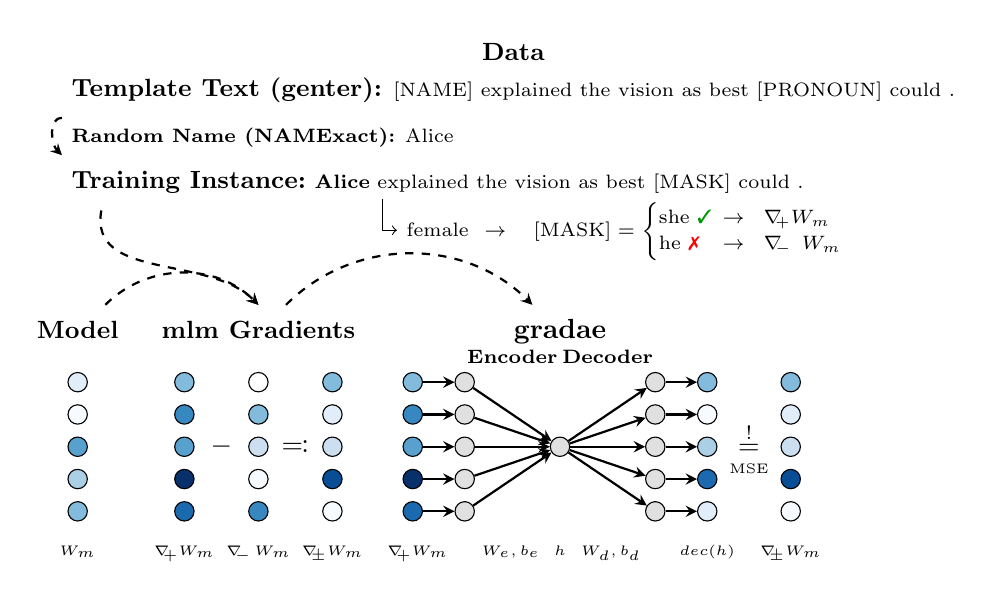
\begin{tikzpicture}[node distance=2cm]

    \edef\neuronHeight{0.15cm}
    \edef\neuronWidth{0.5cm}
    \edef\neuronWidthShort{0.4cm}
    \edef\neuronWidthSum{0.68cm}
    \edef\weightWidth{0.95cm}
    \edef\weightHeight{0.0cm}

    % Define styles
    \tikzstyle{arrow} = [thick,->,>=stealth]

    \tikzstyle{neuron} = [circle, rounded corners, minimum width=7pt, minimum height=7pt, text centered, draw=black, fill=c1, inner sep=0pt]

    \tikzstyle{aeneuron} = [circle, rounded corners, minimum width=7pt, minimum height=7pt, text centered, draw=black, fill=aeneuroncolor, inner sep=0pt]

   \tikzstyle{desc} = [rectangle, rounded corners, minimum width=0.1ex, minimum height=0.1ex, text centered,  text depth=1ex, text height=2ex]

      \tikzstyle{weight} = [rectangle, rounded corners, minimum width=0.1ex, minimum height=0.1ex, text centered,  text depth=1ex, text height=2ex, font=\tiny]

    \tikzstyle{math} = [shape=rectangle, %fill=lightergray, 
    text centered, inner xsep=0ex,  inner ysep=0ex, minimum height=4ex, minimum width=4ex, baseline]


    % BERT
    \node (bert-neuron-1) [neuron, fill=c2] {};
    \node (bert-neuron-2) [neuron, below={\neuronHeight of bert-neuron-1}, fill=c1] {};
    \node (bert-neuron-3) [neuron, below={\neuronHeight of bert-neuron-2}, fill=c6] {};
    \node (bert-neuron-4) [neuron, below={\neuronHeight of bert-neuron-3}, fill=c4] {};
    \node (bert-neuron-5) [neuron, below={\neuronHeight of bert-neuron-4}, fill=c5] {};
    \node (bert-text) [desc, above=\neuronHeight of bert-neuron-1] {\small\textbf{Model}};
    \node (bert-weight) [weight, below={\weightHeight of bert-neuron-5}] {$W_m$};


    \node (mlm-text) [desc, right=0.3cm of bert-text] {\small\textbf{\acrshort{mlm} Gradients}};

    \node (data-text-sample) [desc, xshift=-0.2cm, yshift=3.0cm, anchor=base west] at (bert-text) {\small\textbf{Template Text (\acrshort{genter}):}     \scriptsize{[NAME] explained the vision as best [PRONOUN] could .}};

    \node (data-text) [desc, yshift=0.1cm] at (data-text-sample.north) {\small\textbf{Data}};
    

    \node (data-text-sample-name) [desc,  below=0.9cm of data-text-sample.south west, anchor=base west] {\small\textbf{Training Instance:}\ 
    \scriptsize{\textbf{Alice} explained the vision as best [MASK] could .}};

    \draw[thick, dashed, arrow] (data-text-sample.south west) to[out=180, in=135] (data-text-sample-name.north west);

    \node (female) [desc, below=-0.1cm of data-text-sample-name]{\scriptsize female};
     \draw[->] ($(data-text-sample-name.south) + (-0.7, 0.15)$) |- (female);

     \node (mask) [desc, right=-0.05cm of female] { \scriptsize $\to$ \;\; $\text{[MASK]} = \begin{cases}
        \text{she}  \text{ \cmark} \! \! \! & \to \;\;  \factualnabla W_m \\ \text{he} \text{ \xmark} & \to \;\;  \counterfactualnabla\ W_m 
    \end{cases} $ };

    \node (random-name) [desc, anchor=west] at ($ (data-text-sample.south west)!0.5!(data-text-sample-name.north west) $) 
    {\scriptsize \textbf{Random Name (\namexact):} Alice};

    \draw[thick, dashed, arrow] (data-text-sample-name.south west) ++(0.5, 0) to[out=-100, in=135] (mlm-text.north);


    \node (bert-grad-she-neuron-1) [neuron, fill=c0, below=\neuronHeight of mlm-text] {};
    \node (bert-grad-she-neuron-2) [neuron, fill=c5, below={\neuronHeight of bert-grad-she-neuron-1}] {};
    \node (bert-grad-she-neuron-3) [neuron, fill=c3, below={\neuronHeight of bert-grad-she-neuron-2}] {};
    \node (bert-grad-she-neuron-4) [neuron, fill=c1, below={\neuronHeight of bert-grad-she-neuron-3}] {};
    \node (bert-grad-she-neuron-5) [neuron, fill=c7, below={\neuronHeight of bert-grad-she-neuron-4}] {};
    \node (mlm-she) [weight, xshift=0cm, yshift=0cm, below=\weightHeight of bert-grad-she-neuron-5] {$\counterfactualnabla W_m$};

    \node (bert-grad-he-neuron-1) [neuron, fill=c5, left=\neuronWidthSum of bert-grad-she-neuron-1] {};
    \node (bert-grad-he-neuron-2) [neuron, fill=c7, below={\neuronHeight of bert-grad-he-neuron-1}] {};
    \node (bert-grad-he-neuron-3) [neuron, fill=c6, below={\neuronHeight of bert-grad-he-neuron-2}] {};
    \node (bert-grad-he-neuron-4) [neuron, fill=c10, below={\neuronHeight of bert-grad-he-neuron-3}] {};
    \node (bert-grad-he-neuron-5) [neuron, fill=c8, below={\neuronHeight of bert-grad-he-neuron-4}] {};

    \node (mlm-he) [weight, xshift=0cm, yshift=0cm, below=\weightHeight of bert-grad-he-neuron-5] {$\factualnabla W_m$};

    \node (not-eq) [math] at ($(bert-grad-he-neuron-3.east)!0.5!(bert-grad-she-neuron-3.west)$) {$-$};

    \node (bert-grad-diff-value-1) [neuron, fill=c5, right=\neuronWidthSum of bert-grad-she-neuron-1] {};
    \node (bert-grad-diff-value-2) [neuron, fill=c2, below={\neuronHeight of bert-grad-diff-value-1}] {};
    \node (bert-grad-diff-value-3) [neuron, fill=c3, below={\neuronHeight of bert-grad-diff-value-2}] {};
    \node (bert-grad-diff-value-4) [neuron, fill=c9, below={\neuronHeight of bert-grad-diff-value-3}] {};
    \node (bert-grad-diff-value-5) [neuron, fill=c1, below={\neuronHeight of bert-grad-diff-value-4}] {};

    \node (not-eq) [math, inner xsep=0ex,  % Horizontal padding
                        %inner ysep=0.2ex, % Base vertical padding (for sides)
                        %minimum height=0.3ex, % Force a minimum height for the node
                        %text height=1.4ex, % Adjust top margin
                        %text depth=0.1ex
                        ] at ($(bert-grad-she-neuron-3.east)!0.5!(bert-grad-diff-value-3.west)$) {\raisebox{-0.06em}{$\eqqcolon$}};

   \node (diff) [weight, xshift=0cm, yshift=0cm, below=0.0cm of bert-grad-diff-value-5] 
   %{\small \cmark \!$-$\! \xmark};
    {$\diffnabla W_m$};

    \node (bert-grad-input-neuron-1) [neuron, fill=c5, right=1.7cm of bert-grad-she-neuron-1] {};
    \node (bert-grad-input-neuron-2) [neuron, fill=c7, below={\neuronHeight of bert-grad-input-neuron-1}] {};
    \node (bert-grad-input-neuron-3) [neuron, fill=c6, below={\neuronHeight of bert-grad-input-neuron-2}] {};
    \node (bert-grad-input-neuron-4) [neuron, fill=c10, below={\neuronHeight of bert-grad-input-neuron-3}] {};
    \node (bert-grad-input-neuron-5) [neuron, fill=c8, below={\neuronHeight of bert-grad-input-neuron-4}] {};

    \node (mlm-he2) [weight, xshift=0cm, yshift=0cm, below=0.0cm of bert-grad-input-neuron-5] {\, $\factualnabla W_m$};

    
    \node (ae-input-neuron-1) [aeneuron, right=\neuronWidthShort of bert-grad-input-neuron-1] {};
    \node (ae-input-neuron-2) [aeneuron, below={\neuronHeight of ae-input-neuron-1}] {};
    \node (ae-input-neuron-3) [aeneuron, below={\neuronHeight of ae-input-neuron-2}] {};
    \node (ae-input-neuron-4) [aeneuron, below={\neuronHeight of ae-input-neuron-3}] {};
    \node (ae-input-neuron-5) [aeneuron, below={\neuronHeight of ae-input-neuron-4}] {};
    
    \draw [arrow] (bert-grad-input-neuron-1) -- (ae-input-neuron-1);
    \draw [arrow] (bert-grad-input-neuron-2) -- (ae-input-neuron-2);
    \draw [arrow] (bert-grad-input-neuron-3) -- (ae-input-neuron-3);
    \draw [arrow] (bert-grad-input-neuron-4) -- (ae-input-neuron-4);
    \draw [arrow] (bert-grad-input-neuron-5) -- (ae-input-neuron-5);


    % feature neuron
    \node (ae-latent) [aeneuron, right=\weightWidth of ae-input-neuron-3] {};
        \draw [arrow] (ae-input-neuron-1) -- (ae-latent);
    \draw [arrow] (ae-input-neuron-2) -- (ae-latent);
    \draw [arrow] (ae-input-neuron-3) -- (ae-latent);
    \draw [arrow] (ae-input-neuron-4) -- (ae-latent);
    \draw [arrow] (ae-input-neuron-5) -- (ae-latent);

    \node (ae-input-intermediate) at ($(ae-input-neuron-3)!0.5!(ae-latent)$) {};
    \node (ae-input-weight) [weight] at (ae-input-intermediate|-mlm-he2) {\!$W_e, b_e$};


    \node (ae-output-neuron-3) [aeneuron, right={\weightWidth of ae-latent}] {};
    \node (ae-output-neuron-2) [aeneuron, above={\neuronHeight of ae-output-neuron-3}] {};
    \node (ae-output-neuron-1) [aeneuron, above={\neuronHeight of ae-output-neuron-2}] {};
    \node (ae-output-neuron-4) [aeneuron, below={\neuronHeight of ae-output-neuron-3}] {};
    \node (ae-output-neuron-5) [aeneuron, below={\neuronHeight of ae-output-neuron-4}] {};
    \draw [arrow] (ae-latent) -- (ae-output-neuron-1);
    \draw [arrow] (ae-latent) -- (ae-output-neuron-2);
    \draw [arrow] (ae-latent) -- (ae-output-neuron-3);
    \draw [arrow] (ae-latent) -- (ae-output-neuron-4);
    \draw [arrow] (ae-latent) -- (ae-output-neuron-5);

\node (ae-hidden-weight) [weight] at (ae-latent|-mlm-he2) {$h$};

        \node (ae-output-intermediate) at ($(ae-output-neuron-3)!0.5!(ae-latent)$) {};
    \node (ae-output-weight) [weight] at (ae-output-intermediate|-mlm-he2) {\,\,$W_d, b_d$};
    
    \node (ae-output-value-1) [neuron, fill=c5, right=\neuronWidthShort of ae-output-neuron-1] {};
    \node (ae-output-value-2) [neuron, fill=c1, below={\neuronHeight of ae-output-value-1}] {};
    \node (ae-output-value-3) [neuron, fill=c4, below={\neuronHeight of ae-output-value-2}] {};
    \node (ae-output-value-4) [neuron, fill=c8, below={\neuronHeight of ae-output-value-3}] {};
    \node (ae-output-value-5) [neuron, fill=c2, below={\neuronHeight of ae-output-value-4}] {};
\draw [arrow] (ae-output-neuron-1) -- (ae-output-value-1);
\draw [arrow] (ae-output-neuron-2) -- (ae-output-value-2);
\draw [arrow] (ae-output-neuron-3) -- (ae-output-value-3);
\draw [arrow] (ae-output-neuron-4) -- (ae-output-value-4);
\draw [arrow] (ae-output-neuron-5) -- (ae-output-value-5);

\node (ae-output-value) [weight, below={\weightHeight of ae-output-value-5}] {$dec(h)$}; 


    \node (gradae-text) [desc] at (bert-text-|ae-latent) {\textbf{\acrshort{gradae}}};
    \node (gradae-text-encoder) [desc, font=\footnotesize] at ($(ae-input-neuron-1)!0.5!(gradae-text)$) {\scriptsize\textbf{Encoder}};
\node (gradae-text-decoder) [desc, font=\footnotesize] at ($(ae-output-neuron-1)!0.5!(gradae-text)$) {\scriptsize\textbf{Decoder}};

    \node (bert-grad-diff-target-value-1) [neuron, fill=c5, right=0.8cm of ae-output-value-1] {};
    \node (bert-grad-diff-target-value-2) [neuron, fill=c2, below={\neuronHeight of bert-grad-diff-target-value-1}] {};
    \node (bert-grad-diff-target-value-3) [neuron, fill=c3, below={\neuronHeight of bert-grad-diff-target-value-2}] {};
    \node (bert-grad-diff-target-value-4) [neuron, fill=c9, below={\neuronHeight of bert-grad-diff-target-value-3}] {};
    \node (bert-grad-diff-target-value-5) [neuron, fill=c1, below={\neuronHeight of bert-grad-diff-target-value-4}] {};
       \node (diff) [weight, below={\weightHeight of bert-grad-diff-target-value-5}] 
      % {\small \cmark \!$-$\! \xmark};
      {$\diffnabla W_m$};
      
    \node (not-eq) [math] at ($(ae-output-value-3.east)!0.5!(bert-grad-diff-target-value-3.west)$) {\raisebox{0.56em}{$\overset{!}{=}$}};
    \node (loss) [weight, below=-0.4cm of not-eq] {\tiny MSE}; 

    %\draw[thick, dashed, arrow] ($(bert-grad-diff-target-value-5)!0.5!(ae-output-value-5)$) to[out=270, in=270] ($(ae-input-neuron-4)!0.5!(ae-output-neuron-4)$);

    \draw[thick, dashed, arrow] (bert-text) to[out=45, in=135] (mlm-text.north);
 \draw[thick, dashed, arrow] (mlm-text) to[out=45, in=135] (gradae-text);

    \end{tikzpicture}
   }
\subfigure[Inference Phase: Evaluating the learned feature neuron and changing a models's gender bias.]{
\begin{tikzpicture}
    \edef\neuronHeight{0.15cm}
    \edef\neuronWidth{0.5cm}
    \edef\neuronWidthShort{0.4cm}
    \edef\neuronWidthSum{0.68cm}
    \edef\weightWidth{0.95cm}
    \edef\weightHeight{0.0cm}

    % Define styles
    \tikzstyle{input} = [rectangle, rounded corners, minimum width=3cm, minimum height=1cm, text centered, draw=black, fill=blue]
    \tikzstyle{hidden} = [rectangle, rounded corners, minimum width=3cm, minimum height=1cm, text centered, draw=black, fill=green]
    \tikzstyle{output} = [rectangle, rounded corners, minimum width=3cm, minimum height=1cm, text centered, draw=black, fill=c1]
    \tikzstyle{arrow} = [thick,->,>=stealth]

      \tikzstyle{weight} = [rectangle, rounded corners, minimum width=0.1ex, minimum height=0.1ex, text centered,  text depth=1ex, text height=2ex, font=\tiny]
    
    \tikzstyle{math} = [shape=diamond, draw, text centered, inner xsep=0ex,  inner ysep=0ex, minimum height=4ex, minimum width=4ex, baseline]

    \tikzstyle{neuron} = [circle, rounded corners, minimum width=7pt, minimum height=7pt, text centered, draw=black, fill=c1, inner sep=0pt]

    \tikzstyle{aeneuron} = [circle, rounded corners, minimum width=7pt, minimum height=7pt, text centered, draw=black, fill=aeneuroncolor, inner sep=0pt]

   \tikzstyle{desc} = [rectangle, rounded corners, minimum width=0.1ex, minimum height=0.1ex, text centered,  text depth=1ex, text height=2ex]

   \tikzstyle{desc2} = [rectangle]
    \tikzstyle{math} = [shape=rectangle, text centered, inner xsep=0ex,  inner ysep=0ex, minimum height=4ex, minimum width=4ex, baseline]
    
    % BERT
    \node (bert-neuron-1) [aeneuron, fill=c2] {};
    \node (bert-neuron-2) [aeneuron, below={\neuronHeight of bert-neuron-1}, fill=c1] {};
    \node (bert-neuron-3) [aeneuron, below={\neuronHeight of bert-neuron-2}, fill=c6] {};
    \node (bert-neuron-4) [aeneuron, below={\neuronHeight of bert-neuron-3}, fill=c4] {};
    \node (bert-neuron-5) [aeneuron, below={\neuronHeight of bert-neuron-4}, fill=c5] {};
    \node (bert-text) [desc, above=\neuronHeight of bert-neuron-1] {\small\textbf{Model}};

    \node (bert-weight) [weight, below=\weightHeight of bert-neuron-5] {$W_m$};


\node (lr) [aeneuron, right=\neuronWidthSum of bert-neuron-3, fill=c3] {}; 

    \node (ae-latent) [aeneuron,right=\neuronWidthSum of lr, xshift=-0.2cm] {};

    
    \node (lr-text) [desc2, above=0.3cm of lr, minimum height=0.1cm] {\scriptsize learning rate}; 

    \draw ([yshift=+0.1cm]lr.north) -- ++(0cm,+0.3cm);

    \node (not-eq) [math] at ($(lr.east)!0.5!(ae-latent.west)$) {\large$*$};

    \node (ae-output-neuron-3) [aeneuron, right=\weightWidth of ae-latent] {};
    \node (ae-output-neuron-2) [aeneuron, above={\neuronHeight of ae-output-neuron-3}] {};
    \node (ae-output-neuron-1) [aeneuron, above={\neuronHeight of ae-output-neuron-2}] {};
    \node (ae-output-neuron-4) [aeneuron, below={\neuronHeight of ae-output-neuron-3}] {};
    \node (ae-output-neuron-5) [aeneuron, below={\neuronHeight of ae-output-neuron-4}] {};
        \node (ae-output-intermediate) at ($(ae-output-neuron-3)!0.5!(ae-latent)$) {};
    \node (ae-output-weight) [weight] at (ae-output-intermediate|-mlm-he2) {\,\,$W_d, b_d$};
    \draw [arrow] (ae-latent) -- (ae-output-neuron-1);
    \draw [arrow] (ae-latent) -- (ae-output-neuron-2);
    \draw [arrow] (ae-latent) -- (ae-output-neuron-3);
    \draw [arrow] (ae-latent) -- (ae-output-neuron-4);
    \draw [arrow] (ae-latent) -- (ae-output-neuron-5);
    
    \node (ae-output-value-1) [neuron, fill=c5, right=0.5cm of ae-output-neuron-1] {};
    \node (ae-output-value-2) [neuron, fill=c1, below={\neuronHeight of ae-output-value-1}] {};
    \node (ae-output-value-3) [neuron, fill=c2, below={\neuronHeight of ae-output-value-2}] {};
    \node (ae-output-value-4) [neuron, fill=c9, below={\neuronHeight of ae-output-value-3}] {};
    \node (ae-output-value-5) [neuron, fill=c1, below={\neuronHeight of ae-output-value-4}] {};
\draw [arrow] (ae-output-neuron-1) -- (ae-output-value-1);
\draw [arrow] (ae-output-neuron-2) -- (ae-output-value-2);
\draw [arrow] (ae-output-neuron-3) -- (ae-output-value-3);
\draw [arrow] (ae-output-neuron-4) -- (ae-output-value-4);
\draw [arrow] (ae-output-neuron-5) -- (ae-output-value-5);
 \node (ae-output-value-weight) [weight, below={\weightHeight of ae-output-value-5}] {$dec(h)$};

    \node (gf-text) [desc, below=0.2cm of ae-latent, xshift=-0.0cm] {\scriptsize gender factor}; 
    %\draw[shift={(ae-latent)}] (0,-0.25) -- (gf-text);

    \draw ([yshift=-0.1cm]ae-latent.south) -- ++(0cm,-0.3cm);
    


    \node (lr-math) [weight] at (lr|-bert-weight) {$\alpha$};
    \node (lr-math) [weight] at (ae-latent|-bert-weight) {$h$};
    

    \node (changed-bert-neuron-3) [aeneuron, right={\neuronWidthSum of ae-output-value-3}, fill=c7] {};
    \node (changed-bert-neuron-2) [aeneuron, above={\neuronHeight of changed-bert-neuron-3}, fill=c1] {};
    \node (changed-bert-neuron-1) [aeneuron, above=\neuronHeight of changed-bert-neuron-2, fill=c4] {};
    \node (changed-bert-neuron-4) [aeneuron, below={\neuronHeight of changed-bert-neuron-3}, fill=c8] {};
    \node (changed-bert-neuron-5) [aeneuron, below={\neuronHeight of changed-bert-neuron-4}, fill=c5] {};
    \node (changed-bert-text) [desc, above=\neuronHeight of changed-bert-neuron-1] {\small\textbf{Changed}};
    \node (changed-bert-text2) [desc, below=-0.4cm of changed-bert-text] {\small\textbf{Model}};
    \node (changed-bert-weight) [weight, below=\weightHeight of changed-bert-neuron-5] {$\widetilde{W}_m$};


\node (coloneqq) [math] at ($(ae-output-value-3.east)!0.5!(changed-bert-neuron-3.west)$) {$\eqqcolon$};

\node (plus) [math] at ($(bert-neuron-3.east)!0.5!(lr.west)$) {$+$};

      \node (gradae-text) [desc, xshift=0.55cm] at (bert-text-|ae-latent) {\small\textbf{\acrshort{gradae}}};
    \node (gradae-text-decoder) [desc, font=\footnotesize, xshift=-0.31cm] at ($(ae-output-neuron-1)!0.5!(gradae-text)$)  {\scriptsize\textbf{Decoder}}; 

    
    \node (ae-input-neuron-1) [aeneuron, above=3.95cm of ae-latent, xshift=-0.6cm] {};
    \node (ae-input-neuron-2) [aeneuron, below={\neuronHeight of ae-input-neuron-1}] {};
    \node (ae-input-neuron-3) [aeneuron, below={\neuronHeight of ae-input-neuron-2}] {};
    \node (ae-input-neuron-4) [aeneuron, below={\neuronHeight of ae-input-neuron-3}] {};
    \node (ae-input-neuron-5) [aeneuron, below={\neuronHeight of ae-input-neuron-4}] {};
    
    \node (bert-grad-input-neuron-1) [neuron, fill=c5, left=\neuronWidthShort of ae-input-neuron-1] {};
    \node (bert-grad-input-neuron-2) [neuron, fill=c7, below={\neuronHeight of bert-grad-input-neuron-1}] {};
    \node (bert-grad-input-neuron-3) [neuron, fill=c6, below={\neuronHeight of bert-grad-input-neuron-2}] {};
    \node (bert-grad-input-neuron-4) [neuron, fill=c10, below={\neuronHeight of bert-grad-input-neuron-3}] {};
    \node (bert-grad-input-neuron-5) [neuron, fill=c8, below={\neuronHeight of bert-grad-input-neuron-4}] {};

    \node (mlm-he2) [weight, xshift=0cm, yshift=0cm, below=0.0cm of bert-grad-input-neuron-5] {\, $\factualnabla W_m$};
    
    \draw [arrow] (bert-grad-input-neuron-1) -- (ae-input-neuron-1);
    \draw [arrow] (bert-grad-input-neuron-2) -- (ae-input-neuron-2);
    \draw [arrow] (bert-grad-input-neuron-3) -- (ae-input-neuron-3);
    \draw [arrow] (bert-grad-input-neuron-4) -- (ae-input-neuron-4);
    \draw [arrow] (bert-grad-input-neuron-5) -- (ae-input-neuron-5);


    % feature neuron
    \node (ae-latent2) [aeneuron, right=\weightWidth of ae-input-neuron-3] {};
        \draw [arrow] (ae-input-neuron-1) -- (ae-latent2);
    \draw [arrow] (ae-input-neuron-2) -- (ae-latent2);
    \draw [arrow] (ae-input-neuron-3) -- (ae-latent2);
    \draw [arrow] (ae-input-neuron-4) -- (ae-latent2);
    \draw [arrow] (ae-input-neuron-5) -- (ae-latent2);

    \node (ae-input-intermediate) at ($(ae-input-neuron-3)!0.5!(ae-latent)$) {};
    \node (ae-input-weight) [weight, xshift=-0.6cm] at (ae-latent2|-mlm-he2) {\!$W_e, b_e$};

  \node (gradae-text) [desc, xshift=-0.68cm, above=1cm of ae-latent2] {\small\textbf{\acrshort{gradae}}};
    \node (gradae-text-decoder) [desc, font=\footnotesize, xshift=0.28cm] at ($(ae-input-neuron-1)!0.5!(gradae-text)$)  {\scriptsize\textbf{Encoder}}; 


\node (gradae-text) [desc, xshift=1.48cm, above=1cm of ae-latent2] {\small\textbf{Encoded Value }}; % Interpretation

    \node (gf-text-hint) [desc, right=0.1cm of ae-latent2] {\tiny \tiny$\begin{cases}  >0 & \to \;\; \text{female}\\ =0 & \to \;\; \text{neutral}\\ < 0 & \to \;\; \text{male}\end{cases}$};
\draw[shift={(ae-latent)}] ; %(0,-0.25) -- ++(0, -0.2)
    \node (lr-math) [weight] at (ae-latent2|-ae-input-weight) {$h$};
\end{tikzpicture}

%\caption{Inference Phase: Changing a Models's Gender Bias}
}
    \vspace{-10pt}
    \caption{Our approach - \acrfull{gradae}.}
    \label{fig:gradae}
\end{figure*}


In this section, we introduce a novel approach for targeted feature learning and changing a model's gender bias. 
Our method utilizes a straightforward encoder-decoder architecture that leverages gradient information to encode a gender-related scalar value. This scalar is then decoded into gradient updates, which we believe that they are capable of changing the model's gender bias towards the encoded gender value. An overview of our approach is shown in Figure~\ref{fig:gradae}.

\subsection{Motivation}\label{sec:gradae-motivation}

Gradient-based explanation methods, such as Grad-CAM \citep{gradcam} and Integrated Gradients \citep{integratedGradients}, have proven effective in providing insights into a model's internal workings \cite{chen2020adapting, selvaraju2020grad, lundstrom2022rigorous}, highlighting which parts of the model were crucial to a specific prediction.
%These methods leverage gradients to highlight which parts of the model were crucial to a certain prediction. 
During the training of neural networks, the optimizer inherently determines which neurons require updates, specifically those that contributed incorrectly to the model's output.

We exploit this mechanism by adopting a \gls{mlm} task, a standard pre-training task for transformer language models \cite{bert}. 
Our task involves sentences containing a name, with the masked token corresponding to the gendered pronoun
%third person singular gendered pronoun 
(\emph{he} or \emph{she}).
\begin{quote}
\vspace{-8pt}
    Alice explained the vision as best [MASK] could .
    \vspace{-8pt}
\end{quote}
Gradients are computed for both pronouns as targets:
\begin{quote}
\vspace{-8pt}
\textbf{Factual:} Alice explained the vision as best \emph{she} could . \\
\textbf{Counterfactual:} Alice explained the vision as best \emph{he} could .
\vspace{-8pt}
\end{quote}
This factual-counterfactual evaluation strategy, inspired by \acrshort{crows} \citep{crows}, uses gradient differences to isolate gender-related updates by eliminating non-gender-related changes common to both cases. 
This difference yields two inverse directions: strengthening or mitigating gender bias, depending on the gradient order. 
In the mitigating direction, the factual gender-related updates are eliminated, effectively removing the established factual associations, while the counterfactual updates are emphasized to facilitate the learning of new, counterfactual associations.

\subsection{\acrshort{gradae}}\label{sec:gradae}

In general, we aim to learn how to adjust model parameters to achieve a desired factual or counterfactual state. We hypothesize that the gradients contain the necessary information for this purpose and that the feature changing behavior can be controlled via a learned neuron.

Let $W_m \in \mathbb{R}^n$ denote the $n$ model parameters for which the feature is learned. 
We consider three types of gradients: 
\begin{enumerate*}[label=\textbf{(\arabic*)}]
    \item gradients from the factual masking task~$\factualnabla W_m$,
    \item gradients from the counterfactual masking task~$\counterfactualnabla W_m$,
    and
    \item the difference between these two gradients $\diffnabla W_m \coloneqq \factualnabla W_m - \counterfactualnabla W_m$.
\end{enumerate*}
Here, $\nabla_{\!.}W_m$ represents a vector in $\mathbb{R}^n$, where each component corresponds to the gradient for the parameter at this position.  
We frame the problem as a gradient learning task to predict the gradient difference $\diffnabla W_m$ from the factual gradients $\factualnabla W_m$: %, formally:
\begin{equation*}
    \text{Learn } f  \text{ s.t. } f(\factualnabla W_m) \approx \diffnabla W_m.
\end{equation*}
For this study, we propose a simple encoder-decoder structure $f = dec \circ enc$, where:
\begin{align*}
    enc(\factualnabla W_m) &= \tanh(W_e^T \cdot \factualnabla W_m + b_e) && \eqqcolon h \in \mathbb{R}, \\
    dec(h) &= h \cdot W_d + b_d && \approx \diffnabla W_m.
\end{align*}
Here, $W_e, W_d, b_d\in \mathbb{R}^n$ and $b_e\in \mathbb{R}$ are learnable parameters, resulting in a total of $3n+1$ parameters. We refer to this approach as \gls{gradae}.


\begin{table*}[!t]
    \centering
    \caption{Overview of datasets including total number of samples and a description.}
    \label{tab:dataset-summary}
    \begin{tabularx}{\textwidth}{lrX}
    \toprule 
         \textbf{Name}  & \textbf{Size} & \textbf{Description}\\ 
         \midrule
        \namexact & 1,398 & Names that are unambiguous (\emph{exact}) in meaning and gender, e.g., \emph{Alice, Bob, Eve} \\     
        \namextend \! & 40,351 & Extends \namexact\ with less certain names, including those with multiple meanings and genders,
        e.g.,  \emph{Alice, Bob, Christian, Drew, Eve, Florence, Skyler} \\
        \acrshort{genter} & 27,031 & Name-gender templates, 
        e.g., \emph{[NAME] explained the vision as best [PRONOUN] could .} \\ 
        \acrshort{geneutral} & \!\!\!\! 7,896,455 & Contains only gender-neutral words, e.g., 
        \emph{i really want to see you again , soon if you can .}
        \\
        \acrshort{gentypes} & 500 & Gender-stereotypical templates, 
        e.g., \emph{My friend, [NAME], loves taking care of babies.} \\
         \bottomrule
    \end{tabularx}
\end{table*}

\subsection{\gradae\ for Gender Debiasing}\label{sec:gradae-for-gender-debiasing}
While \gradae\ is defined to work with binary features in general, we restrict the following proof of concept to gender.
In this setup, \ref{item:hyp1} suggests that using the proposed factual and counterfactual masking tasks guides the encoder to encode a gender-related scalar feature $h$, indicating that the factual gradients contain gender-specific information.
\ref{item:hyp3} asserts that $dec(h)$ can be used to adjust the model's gender bias, e.g., by choosing a specific \emph{gender factor} $h$ and \emph{learning rate} $\alpha$ to update the model parameters as follows:
\[\widetilde{W}_m \coloneqq W_m + \alpha \cdot dec(h).\] 
Experiments show that gender-related inputs are mostly mapped to values close to $-1$ and $+1$, corresponding to male and female gender or vice versa. 
WLOG, we assume positive values represent the female and negative values the male gender, and we modify the model accordingly to standardize the results for simplified definitions and consistent visualizations.


\section{Data}

The training and evaluation of \gradae\ relies on specialized data summarized in Table~\ref{tab:dataset-summary}.
The datasets include two name collections (\namexact\ and \namextend), a dataset linking names to gender through masked pronouns (\genter), a dataset of exclusively gender-neutral text (\geneutral), and a dataset associating masked names with gender stereotypes (\gentypes). We split the datasets used for training (\genter\ and \namexact) in \emph{train}/\emph{val}/\emph{test} sets, and denote a specific split of a dataset by an index, e.g., \namexacttrain.
Detailed descriptions of dataset generation can be found in Appendix~\ref{app:data}. 


\section{Metrics}

In this section, we introduce the metrics utilized for evaluating \gls{gradae} in learning a gender feature neuron and applying it for debiasing using this neuron.

\subsection{Encoder as Gender Classifier}\label{sec:metrics:enc}

Following~\ref{item:hyp1}, we evaluate whether the \gradae\ encoder encodes gender-related information by treating it as gender classifier. 
\genter\ is used as labeled data, with $+1$ for female gradients and $-1$ for male ones.
To measure how well the encoded values distinguish between genders, we compute the Pearson correlation coefficient \cite{pearson},
denoted as \cormf, between the labels and the encoded values. Additionally, we compute the balanced accuracy, denoted as \accmf, where positive encoded values are classified as female and as male otherwise. 

An encoded value of $0$ can be seen as a neutral class,, representing a natural midpoint between the male and female extremes. For datasets with labels $\pm 1$ for gender and $0$ for gender-neutral texts, we calculate again both, correlation and balanced accuracy. In this case, values $\ge 0.5$ are classified female, $\le -0.5$ as male, and intermediate values as neutral. Specifically, these three-label-metrics are computed across a combination of three datasets:
\begin{itemize}
\vspace{-8pt}
    \item \genter: Labeled as $\pm1$ as before for \cormf. %\ and \accmf.
    \vspace{-5pt}
    \item \genterzero: A variation of \genter\ where instead of the pronoun, a random gender-neutral token is chosen for masking and target calculation, considering a sentence of \genter\ with a valid name/pronoun pair. This evaluates gender classification in a similar setting to training but with non-gender-related masking.
    \vspace{-5pt}
    \item \geneutral: A dataset where all tokens are gender-neutral by design, with a single token chosen for masking and target calculation.
    \vspace{-5pt}
\end{itemize}

\genter\ provides labels $\pm 1$, while the others contribute only labels $0$. Across all three datasets, we compute the correlation, \corenc, and the balanced accuracy, \accenc. 
We also calculate the mean absolute encoded value $h$ for each dataset, denoted as \mamf, \masmf, and \man.

\subsection{Gender Bias Changed Models}\label{sec:metrics:dec}
We introduce metrics to quantify gender bias in a base model. Specifically, we aim to measure how debiased, female-biased or male-biased a model is. To achieve this, we define several intermediate metrics. These are informally introduced here and formally defined in Appendix~\ref{app:metrics}.

Let $F$ represent the female gender, $M$ represent the male gender, and $G\in\{F, M\}$ denote a gender. Let $t$ be a text of \gentypes, i.e., a stereotyped sentence whose masked token intuitively matches well with names. The considered metrics are as follows:
\begin{enumerate*}[label=\textbf{(\arabic*)}]
\item \accdec\ is an accuracy score for an \gls{mlm} task over \geneutral, i.e., data independent of gender, used to evaluate the model's general language modeling capabilities.

\item $\P_t(G)$ denotes the probability of $G$ for task $t$, defined as the sum of all probabilities belonging to single token names of that gender considering the \gls{mlm} task~$t$. 

\item $\P(G)$ is the average probability of $G$, i.e., $\P_t(G)$ averaged over all $t$ in \gentypes.
 
\item The \gls{bpi} quantifies a model's gender bias by combining  
high $\accdec$ to ensure good language modeling capabilities, 
balanced gender probabilities ($|\P_t(F)-\P_t(M)|$ is low) to ensure a low gender bias, 
and high overall reasonable predictions ($\P_t(M) + \P_t(F)$ is high).

\item The \gls{fpi} measures bias towards the female gender by favoring models with high $\accdec$, low $\P_t(M)$, and high $\P_t(F)$.

\item Similarly, the \gls{mpi} measures bias towards the male gender. 
\end{enumerate*}

The purpose of the last three metrics is to select the most debiased, female-biased, and male-biased models from a set of candidates, as discussed in Section~\ref{sec:eval-decoder}.


\section{Evaluation}\label{sec:evaluation}

In this section, we evaluate four \glspl{gradae}: two based on BERT \cite{bert} (\bertbase\ and \bertlarge), one large \roberta\ \cite{roberta}, and one small \mbox{\distilbert} \cite{distilbert} model. 
These models represent different variants of encoder-only architectures, including the lightweight \distilbert.
For simplicity, all metrics are reported for the test split (or the entire dataset if not split), unless stated otherwise. 
For example, \cormf\ is \cormftest\ and \cormfval\ refers to the \cormf\ metric for \genterval.



\subsection{Training}\label{sec:eval-training}

For each base model, we trained three \glspl{gradae} with different random seeds, selecting the best model based on \cormfval\ at the end of the training process. 
Importantly, the prediction layers were excluded from \gradae\ parameters to ensure debiasing targets the language model itself, not just the classification head.
In each training step, a batch is processed with a uniformly randomly selected gender, sampling only names of that gender from  \namexacttrain\ and pairing them with sentences from \gentertrain. 
In total, we perform 23,653 training steps, corresponding to the number of template sentences in \gentertrain.
Further details about the training setup are provided in Appendix~\ref{app:training}.


\subsection{Encoder as Gender Classifier}\label{sec:eval-encoder}


\begin{table*}[!t]
    \centering
    \caption{Evaluation of the encoder of various \gradae\ models.}
    \label{tab:encoded_values_cor}
    \begin{tabular}{lrrrrrrr}
    \toprule
         \textbf{Model} & \textbf{\accenc} & \textbf{\corenc} & \textbf{\accmf} &  \textbf{\cormf} & \textbf{\mamf} & \textbf{\masmf} & \textbf{\man}  \\\midrule
\bertbase  &              0.612 &              0.669 &             1.000 &             0.957 &            0.853 &            0.431 &           0.369 \\
 \bertlarge &              0.578 &              0.616 &             1.000 &             0.908 &            0.725 &            0.399 &           0.340 \\
 \distilbert      &              0.758 &              0.838 &             1.000 &             1.000 &            0.999 &            0.321 &           0.242 \\
  \roberta         &              0.909 &              0.935 &             1.000 &             1.000 &            1.000 &            0.130 &           0.132 \\
          \bottomrule
    \end{tabular}
\end{table*}

We analyze the scalar encoded value of the \gls{gradae} models in Figure~\ref{fig:encoded-values} and Table~\ref{tab:encoded_values_cor} to evaluate \ref{item:hyp1}. % and \ref{item:hyp2}. 
We use three different datasets (see Section~\ref{sec:metrics:enc}):
\begin{enumerate*}[label=\textbf{\arabic*)}] \item For \gentertest, we perform gendered masking by pairing each template with one male and one female name from \namexacttest, resulting in 5,406 samples.\label{item:genter} \item In \genterzero, we use the same data as in~\ref{item:genter}, but with non-gender-specific tokens masked. \item For \geneutral, we perform masking on 10,000 samples. \end{enumerate*}
\begin{figure}[!t]
    \centering
    \includegraphics[width=\linewidth]{img/encoded_values_bertbase_bertlarge_distilbert_roberta.pdf}
    \vspace{-20pt}
    \caption{Distribution of the encoded value for different datasets and \gls{gradae} models.}
    \label{fig:encoded-values}
    % export.encoder_plot()
    \vspace{-5pt}
\end{figure}
As shown in Figure~\ref{fig:encoded-values}, all models encode primarily values of $-1$ and $+1$ for gender-specific masking. For non-gender-specific masking, encoded values tend to center around a neutral value of $0.0$, though the classification is less precise compared to gender-related masking. Importantly, the non-gender-specific masks were not seen during training.

Table~\ref{tab:encoded_values_cor} quantifies these observations. When only gender-specific data is considered (\accmf\ and \cormf), the encoder distinguishes the input classes almost perfectly. However, when neutral inputs are included (\accenc\ and \corenc), which were not encountered during training, the task becomes more difficult, and the results are less accurate. 
Interestingly, \bertlarge\ and \bertbase\ perform similarly, both surpassed by \distilbert, while \roberta\ outperforms even \distilbert, especially on gender-neutral inputs.

\hypresult{The \gradae\ models successfully learned a feature neuron with the desired interpretation (gender), supporting \ref{item:hyp1}.}


\subsection{Decoder as Bias-Changer}\label{sec:eval-decoder}

% export.changed_model_selection.py
\generateModelPlotsSmallSquare{bert}{\bertbase}

In this section, we investigate how the learned representation of the decoder can change the model’s bias.
The adjustment is controlled by two key parameters: the scalar input to the decoder network $h$ (called \emph{gender factor}) and the \emph{learning rate} $\alpha$, which determines the scaling of the decoder output before adding it to the model weights.
To assess the impact of these parameters, we evaluate the \gradae\ models across a grid of 15 gender factors and 16 learning rates, modifying the model weights as $\widetilde{W_m} \coloneqq W_m + \alpha \cdot dec(h)$. The results for \bertbase\ are shown in Figure~\ref{fig:changed_models-bert}, with additional plots for the other base models provided in Appendix~\ref{app:decoder-as-bias-changer}.


Interestingly, all plots exhibit a nearly point-symmetric behavior. Due to the simplicity of the \gradae\ decoder architecture, the only difference between cells with inverted gender factor and learning rate is twice the bias term $b_e$, which becomes less influential as the gender factor grows.

Specifically, for $\P(F)$ (Figure~\ref{fig:changed_models-bert:prob_f}) and $\P(M)$ (Figure~\ref{fig:changed_models-bert:prob_m}) show an inverse pattern.
The normalization of the encoder and the definition of $\diffnabla W_m$ (Section~\ref{sec:gradae}) result in a consistent pattern across all models: when the signs of $h$ and $\alpha$ are equal, the model biases toward male, whereas different signs lead to a bias toward female.
\accdec\ (Figure~\ref{fig:changed_models-bert:acc}) reveals a broad region of high probability, provided the learning rate remains moderate.

Figures~\ref{fig:changed_models-bert:bpi} to~\ref{fig:changed_models-bert:mpi} illustrate the optimal models for \gls{bpi}, \gls{fpi}, and \gls{mpi}, respectively. Colored arrows in the subplot captions illustrate how each sub-metric influences the aggregated metrics. 
Visually, these figures capture the trade-offs inherent in this debiasing approach, similar to those observed in other studies \cite{movementPruning}. 
These aggregated metrics demonstrate that while stronger bias modification degrades language modeling performance, a \emph{safe region} exists with moderate gender factors and learning rates.
Considering the \gls{bpi} plot (Figure~\ref{fig:changed_models-bert:bpi}) and gender factor $h=0.0$, the \gradae\ decoder's bias vector $b_e$ effectively learned an appropriate debiasing direction.

Based on \gls{bpi}, \gls{fpi}, and \gls{mpi}, we identify models that are well-suited for defining debiased, female, and male representations, respectively.
Table~\ref{tab:eval:own-metrics} lists the parameters and metrics for the selected models across all base models.

Surprisingly, for the \roberta\ base model, $\P(F)>\P(M)$ holds true, unlike all other base models. 
This indicates a female bias in the given task, contradicting our expectation that language models typically exhibit male bias (although this bias direction is not captured by \gls{ss}, \gls{seat}, and \gls{crows}). 

Interestingly, the difference in \gls{bpi} between \gradiendbpi\ and its base model is relatively small, whereas the corresponding differences for \gls{fpi} and \gls{mpi} are much larger, respectively. 
This observation suggests that biasing a model (in either direction) is easier than debiasing it.
Notably, \gls{fpi} approaches nearly zero for \gradiendmpi\ models, and \gls{mpi} similarly is close to zero for \gradiendfpi\ models.

\begin{table*}[!t]% export.changed_model_selection.py
    \centering
    \caption{Selected debiased, female-biased and male-biased models based on \gls{bpi}, \gls{fpi} and \gls{mpi}.}\label{tab:eval:own-metrics}
\begin{tabular}{lrrrrrrrr}
\toprule
 \textbf{Model}    & \textbf{GF} $h$   & \textbf{LR} $\alpha$   & \textbf{$\mathbb{P}(F)$}   & \textbf{$\mathbb{P}(M)$}   & \textbf{\accdec}   & \textbf{BPI}   & \textbf{FPI}   & \textbf{MPI}   \\
\midrule
 \bertbase         & 0.0               & 0.0                    & 0.413                      & 0.538                      & 0.496              & 0.322          & 0.110          & 0.172          \\
 \, + \gradiendbpi & 0.0               & 1e-02                  & 0.424                      & 0.494                      & 0.491              & 0.363          & 0.111          & 0.145          \\
 \, + \gradiendfpi & 1.0               & -1e-02                 & 0.948                      & 0.034                      & 0.490              & 0.041          & 0.449          & 0.001          \\
 \, + \gradiendmpi & -1.0              & -1e-02                 & 0.031                      & 0.940                      & 0.490              & 0.043          & 0.001          & 0.446          \\
\midrule
 \bertlarge        & 0.0               & 0.0                    & 0.432                      & 0.534                      & 0.511              & 0.280          & 0.132          & 0.184          \\
 \, + \gradiendbpi & -0.2              & 5e-02                  & 0.461                      & 0.434                      & 0.486              & 0.397          & 0.128          & 0.115          \\
 \, + \gradiendfpi & 0.6               & -5e-02                 & 0.960                      & 0.031                      & 0.508              & 0.036          & 0.473          & 0.001          \\
 \, + \gradiendmpi & -0.4              & -5e-02                 & 0.024                      & 0.963                      & 0.511              & 0.031          & 0.000          & 0.480          \\
\midrule
 \distilbert       & 0.0               & 0.0                    & 0.307                      & 0.361                      & 0.392              & 0.230          & 0.075          & 0.096          \\
 \, + \gradiendbpi & -1.0              & 5e-04                  & 0.358                      & 0.320                      & 0.386              & 0.231          & 0.092          & 0.078          \\
 \, + \gradiendfpi & 0.8               & -1e-02                 & 0.724                      & 0.045                      & 0.350              & 0.080          & 0.241          & 0.004          \\
 \, + \gradiendmpi & 0.0               & -5e-02                 & 0.036                      & 0.599                      & 0.384              & 0.092          & 0.005          & 0.221          \\
\midrule
 \roberta          & 0.0               & 0.0                    & 0.555                      & 0.404                      & 0.573              & 0.208          & 0.249          & 0.162          \\
 \, + \gradiendbpi & 0.4               & 1e-01                  & 0.402                      & 0.499                      & 0.560              & 0.354          & 0.127          & 0.181          \\
 \, + \gradiendfpi & 0.4               & -5e-01                 & 0.980                      & 0.016                      & 0.539              & 0.019          & 0.520          & 0.000          \\
 \, + \gradiendmpi & -1.0              & -1e-01                 & 0.023                      & 0.966                      & 0.568              & 0.032          & 0.001          & 0.535          \\
\bottomrule
\end{tabular}
\end{table*}


\hypresult{The \gradae\ decoder is capable of changing the model's gender bias, confirming \ref{item:hyp3}.}
\vspace{-10pt}


\subsection{Comparison to Other Debiasing Techniques}\label{sec:eval-debiased}

\begin{table*}[!t]
\centering
\caption{Comparison of bootstrapped gender-bias-metrics (\acrshort{ss}, \acrshort{seat}, and CrowS) and language modeling metrics (\acrshort{lms} and \acrshort{glue}) across different debiasing techniques. Statistically significant improvements are indicated in \emph{italics}, while the best score for each base model is highlighted in \textbf{bold}.}\label{tab:eval:main-results}
\tiny
\begin{tabular}{lrrrrr}
\toprule\textbf{Model} & \textbf{\acrshort{ss}} (\%) \bestatfiftytiny & \textbf{\acrshort{seat}} \bestatzerotiny & \textbf{CrowS} (\%) \bestatfiftytiny & \textbf{\acrshort{lms}} (\%) $\uparrow$ & \textbf{\acrshort{glue}} (\%) $\uparrow$\\
\midrule
\bertbase &  $61.24 \pm 1.89$ &  $0.61 \pm 0.29$ &  $54.42 \pm 6.05$ &  $82.50 \pm 0.81$ &  $77.59 \pm 1.18$\\
\lightcmidrule{1-6}
\, + \gradiendbpi & \da{$0.75$} $60.49 \pm 1.93$ & \da{$0.10$} $0.51 \pm 0.19$ & \da{$0.01$} $54.40 \pm 5.98$ & \dab{$0.41$} $82.09 \pm 0.81$ & \dab{$0.08$} $77.51 \pm 1.08$\\
\, + \gradiendfpi & \da{$2.29$} $58.95 \pm 1.96$ & \ua{$0.19$} $0.79 \pm 0.24$ & \da{$3.37$} $51.05 \pm 6.13$ & \dab{$0.22$} $82.28 \pm 0.81$ & \dab{$0.10$} $77.49 \pm 1.12$\\
\, + \gradiendmpi & \da{$1.38$} $59.86 \pm 1.94$ & \da{$0.18$} $0.43 \pm 0.16$ & \da{$0.90$} $46.48 \pm 6.11$ & \uag{$0.39$} $82.89 \pm 0.80$ & \dab{$0.23$} $77.36 \pm 1.09$\\
\lightcmidrule{1-6}
\, + \cda & \da{$2.10$} $59.14 \pm 1.96$ & \da{$0.21$} $0.40 \pm 0.20$ & \da{$1.38$} $53.04 \pm 6.03$ & \uag{$0.58$} $83.07 \pm 0.81$ & \dab{$0.15$} $77.44 \pm 1.04$\\
\, + \dropout & \da{$1.49$} $59.75 \pm 1.93$ & \da{$0.16$} $0.45 \pm 0.25$ & \da{$0.45$} $53.97 \pm 5.98$ & \dab{$\mathit{1.75}$} $\mathit{80.75} \pm \mathit{0.83}$ & \dab{$1.31$} $76.28 \pm 1.22$\\
\, + \inlp & \!\!\da{$\boldsymbol{\mathit{6.24}}$} $\mathit{\boldsymbol{\mathit{55.00}}} \pm \mathit{1.99}$ & \da{$0.24$} $0.37 \pm 0.19$ & \ua{$3.41$} $57.83 \pm 5.96$ & \!\!\uag{$\boldsymbol{1.18}$} $\mathbf{83.68} \pm 0.80$ & \!\!\uag{$\boldsymbol{0.78}$} $\mathbf{78.37} \pm 1.27$\\
\, + \selfdebias & \da{$1.19$} $60.05 \pm 1.94$ & - & \da{$3.96$} $49.55 \pm 6.06$ & \dab{$0.02$} $82.47 \pm 0.83$ & -\\
\, + \sentencedebias & \da{$1.06$} $60.18 \pm 1.91$ & \da{$0.27$} $0.34 \pm 0.13$ & \da{$2.28$} $52.14 \pm 5.99$ & \dab{$0.01$} $82.49 \pm 0.81$ & \uag{$0.00$} $77.59 \pm 1.18$\\
\lightcmidrule{1-6}
\, + \gradiendbpi\ + \inlp & \da{$\mathit{6.17}$} $\mathit{55.07} \pm \mathit{1.97}$ & \!\!\da{$\boldsymbol{0.31}$} $\mathbf{0.30} \pm 0.12$ & \ua{$1.91$} $56.33 \pm 6.04$ & \uag{$0.81$} $83.31 \pm 0.79$ & \dab{$0.23$} $77.36 \pm 1.11$\\
\, + \gradiendbpi\ + \sentencedebias \!\! & \da{$1.59$} $59.65 \pm 1.95$ & \da{$0.18$} $0.43 \pm 0.14$ & \!\!\da{$\boldsymbol{4.16}$} $\mathbf{50.25} \pm 6.14$ & \dab{$0.44$} $82.06 \pm 0.82$ & \dab{$0.11$} $77.47 \pm 1.08$\\

\midrule
\bertlarge &  $61.26 \pm 1.89$ &  $0.52 \pm 0.26$ &  $53.51 \pm 6.05$ &  $82.89 \pm 0.80$ &  $79.59 \pm 0.95$\\
\lightcmidrule{1-6}
\, + \gradiendbpi & \da{$\mathit{5.61}$} $\mathit{55.65} \pm \mathit{1.97}$ & \ua{$0.03$} $0.55 \pm 0.13$ & \!\!\da{$\boldsymbol{3.16}$} $\mathbf{50.35} \pm 6.12$ & \dab{$1.31$} $81.58 \pm 0.83$ & \uag{$0.49$} $80.09 \pm 0.88$\\
\, + \gradiendfpi & \da{$1.11$} $60.15 \pm 1.89$ & \ua{$\mathit{0.58}$} $\mathit{1.10} \pm \mathit{0.13}$ & \da{$0.29$} $53.22 \pm 6.14$ & \dab{$0.82$} $82.06 \pm 0.79$ & \dab{$0.15$} $79.45 \pm 0.95$\\
\, + \gradiendmpi & \da{$1.59$} $59.67 \pm 1.91$ & \da{$0.14$} $0.38 \pm 0.16$ & \da{$3.02$} $49.51 \pm 6.01$ & \dab{$0.38$} $82.50 \pm 0.80$ & \uag{$0.57$} $80.16 \pm 0.90$\\
\lightcmidrule{1-6}
\, + \cda & \da{$2.00$} $59.26 \pm 1.96$ & \ua{$0.11$} $0.63 \pm 0.24$ & \ua{$0.52$} $54.03 \pm 6.21$ & \!\!\uag{$\boldsymbol{0.69}$} $\mathbf{83.57} \pm 0.79$ & \uag{$0.04$} $79.63 \pm 0.86$\\
\, + \dropout & \da{$2.44$} $58.82 \pm 1.94$ & \ua{$0.17$} $0.69 \pm 0.22$ & \ua{$2.11$} $55.62 \pm 6.07$ & \dab{$\mathit{2.57}$} $\mathit{80.32} \pm \mathit{0.82}$ & \dab{$0.70$} $78.89 \pm 0.96$\\
\, + \inlp & \da{$1.93$} $59.33 \pm 1.93$ & \da{$0.23$} $0.29 \pm 0.15$ & \da{$1.39$} $52.12 \pm 5.94$ & \uag{$0.52$} $83.41 \pm 0.79$ & \uag{$0.43$} $80.03 \pm 1.27$\\
\, + \selfdebias & \da{$1.24$} $60.02 \pm 1.91$ & - & \da{$0.35$} $53.16 \pm 6.00$ & \dab{$0.31$} $82.58 \pm 0.81$ & -\\
\, + \sentencedebias & \da{$1.41$} $59.85 \pm 1.91$ & \!\!\da{$\boldsymbol{0.29}$} $\mathbf{0.23} \pm 0.14$ & \da{$2.60$} $50.91 \pm 6.00$ & \dab{$0.09$} $82.80 \pm 0.81$ & \uag{$0.38$} $79.97 \pm 0.91$\\
\lightcmidrule{1-6}
\, + \gradiendbpi\ + \inlp & \!\!\da{$\boldsymbol{\mathit{5.74}}$} $\mathit{\boldsymbol{\mathit{55.52}}} \pm \mathit{1.97}$ & \da{$0.21$} $0.31 \pm 0.13$ & \da{$2.82$} $50.69 \pm 5.95$ & \uag{$0.19$} $83.07 \pm 0.80$ & \uag{$0.04$} $79.64 \pm 0.89$\\
\, + \gradiendbpi\ + \sentencedebias \!\! & \da{$\mathit{5.29}$} $\mathit{55.97} \pm \mathit{1.98}$ & \da{$0.04$} $0.48 \pm 0.13$ & \da{$1.50$} $47.99 \pm 5.98$ & \dab{$1.17$} $81.72 \pm 0.83$ & \!\!\uag{$\boldsymbol{0.65}$} $\mathbf{80.25} \pm 0.90$\\

\midrule
\distilbert &  $59.24 \pm 1.95$ &  $0.80 \pm 0.24$ &  $56.83 \pm 5.99$ &  $82.06 \pm 0.80$ &  $74.09 \pm 1.11$\\
\lightcmidrule{1-6}
\, + \gradiendbpi & \da{$0.40$} $58.84 \pm 1.97$ & \da{$0.00$} $0.80 \pm 0.24$ & \da{$2.68$} $54.15 \pm 6.18$ & \dab{$0.06$} $82.01 \pm 0.80$ & \uag{$0.04$} $74.13 \pm 1.12$\\
\, + \gradiendfpi & \da{$3.20$} $56.05 \pm 1.96$ & \da{$0.01$} $0.80 \pm 0.22$ & \da{$5.64$} $48.81 \pm 6.12$ & \dab{$0.98$} $81.08 \pm 0.81$ & \uag{$0.22$} $74.32 \pm 1.15$\\
\, + \gradiendmpi & \ua{$2.58$} $61.82 \pm 1.90$ & \ua{$0.27$} $1.07 \pm 0.25$ & \da{$6.04$} $50.78 \pm 5.97$ & \dab{$0.28$} $81.79 \pm 0.83$ & \uag{$0.01$} $74.10 \pm 1.16$\\
\lightcmidrule{1-6}
\, + \cda & \da{$1.95$} $57.29 \pm 2.03$ & \da{$0.06$} $0.74 \pm 0.21$ & \da{$3.12$} $53.71 \pm 6.07$ & \!\!\uag{$\boldsymbol{0.23}$} $\mathbf{82.29} \pm 0.80$ & \uag{$0.11$} $74.21 \pm 1.14$\\
\, + \dropout & \ua{$3.17$} $62.41 \pm 1.97$ & \da{$0.02$} $0.78 \pm 0.26$ & \!\!\da{$\boldsymbol{6.05}$} $\mathbf{49.23} \pm 6.04$ & \dab{$\mathit{1.82}$} $\mathit{80.24} \pm \mathit{0.85}$ & \!\!\uag{$\boldsymbol{0.48}$} $\mathbf{74.57} \pm 1.18$\\
\, + \inlp & \da{$\mathit{4.03}$} $\mathit{55.21} \pm \mathit{2.03}$ & \da{$0.18$} $0.62 \pm 0.13$ & \da{$4.36$} $47.54 \pm 5.98$ & \dab{$0.52$} $81.55 \pm 0.79$ & \dab{$0.36$} $73.73 \pm 1.21$\\
\, + \selfdebias & \ua{$0.89$} $60.13 \pm 1.92$ & - & \da{$4.47$} $52.35 \pm 6.25$ & \dab{$0.40$} $81.67 \pm 0.82$ & -\\
\, + \sentencedebias & \da{$2.32$} $56.92 \pm 1.99$ & \!\!\da{$\boldsymbol{0.22}$} $\mathbf{0.58} \pm 0.12$ & \da{$5.98$} $49.16 \pm 5.97$ & \dab{$0.06$} $82.01 \pm 0.80$ & \uag{$0.15$} $74.25 \pm 1.14$\\
\lightcmidrule{1-6}
\, + \gradiendbpi\ + \inlp & \!\!\da{$\boldsymbol{\mathit{5.17}}$} $\mathit{\boldsymbol{\mathit{54.07}}} \pm \mathit{2.03}$ & \da{$0.18$} $0.62 \pm 0.13$ & \da{$5.47$} $48.64 \pm 5.89$ & \dab{$0.61$} $81.46 \pm 0.79$ & \dab{$0.10$} $73.99 \pm 1.23$\\
\, + \gradiendbpi\ + \sentencedebias \!\! & \da{$3.08$} $56.16 \pm 2.01$ & \!\!\da{$\boldsymbol{0.22}$} $\mathbf{0.58} \pm 0.12$ & \da{$5.66$} $48.84 \pm 5.94$ & \dab{$0.13$} $81.93 \pm 0.80$ & \uag{$0.34$} $74.43 \pm 1.12$\\

\midrule
\roberta &  $66.80 \pm 1.88$ &  $0.58 \pm 0.17$ &  $60.01 \pm 5.85$ &  $89.09 \pm 0.64$ &  $77.63 \pm 1.29$\\
\lightcmidrule{1-6}
\, + \gradiendbpi & \da{$2.91$} $63.89 \pm 1.90$ & \da{$0.10$} $0.48 \pm 0.13$ & \da{$6.21$} $53.80 \pm 5.92$ & \dab{$0.27$} $88.82 \pm 0.66$ & \dab{$\mathit{2.50}$} $\mathit{75.13} \pm \mathit{1.19}$\\
\, + \gradiendfpi & \da{$\mathit{4.16}$} $\mathit{62.64} \pm \mathit{1.91}$ & \ua{$\mathit{0.28}$} $\mathit{0.86} \pm \mathit{0.10}$ & \da{$5.79$} $54.22 \pm 6.14$ & \dab{$\mathit{2.58}$} $\mathit{86.51} \pm \mathit{0.71}$ & \dab{$\mathit{3.42}$} $\mathit{74.21} \pm \mathit{1.32}$\\
\, + \gradiendmpi & \da{$0.64$} $66.16 \pm 1.85$ & \da{$0.17$} $0.41 \pm 0.15$ & \da{$9.15$} $50.86 \pm 5.83$ & \dab{$0.13$} $88.95 \pm 0.64$ & \uag{$1.52$} $79.15 \pm 1.24$\\
\lightcmidrule{1-6}
\, + \cda & \da{$2.85$} $63.94 \pm 1.92$ & \da{$0.13$} $0.45 \pm 0.14$ & \da{$0.78$} $59.23 \pm 5.92$ & \uag{$0.02$} $89.11 \pm 0.65$ & \!\!\uag{$\boldsymbol{2.25}$} $\mathbf{79.88} \pm 1.13$\\
\, + \dropout & \!\!\da{$\boldsymbol{\mathit{6.46}}$} $\mathit{\boldsymbol{\mathit{60.33}}} \pm \mathit{1.92}$ & \da{$0.08$} $0.49 \pm 0.12$ & \da{$4.13$} $55.88 \pm 6.03$ & \dab{$\mathit{3.74}$} $\mathit{85.34} \pm \mathit{0.72}$ & \dab{$\mathit{12.19}$} $\mathit{65.44} \pm \mathit{1.06}$\\
\, + \inlp & \da{$\mathit{4.09}$} $\mathit{62.71} \pm \mathit{1.94}$ & \da{$0.14$} $0.44 \pm 0.14$ & \da{$8.91$} $48.90 \pm 5.79$ & \dab{$0.01$} $89.08 \pm 0.63$ & \uag{$\mathit{2.13}$} $\mathit{79.76} \pm \mathit{0.78}$\\
\, + \selfdebias & \da{$1.79$} $65.00 \pm 1.90$ & - & \da{$4.92$} $55.09 \pm 5.79$ & \dab{$0.47$} $88.62 \pm 0.65$ & -\\
\, + \sentencedebias & \da{$1.92$} $64.88 \pm 1.89$ & \da{$0.09$} $0.49 \pm 0.14$ & \da{$6.48$} $53.53 \pm 5.95$ & \uag{$0.05$} $89.14 \pm 0.63$ & \uag{$0.63$} $78.25 \pm 1.10$\\
\lightcmidrule{1-6}
\, + \gradiendbpi\ + \inlp & \da{$\mathit{6.29}$} $\mathit{60.51} \pm \mathit{1.85}$ & \!\!\da{$\boldsymbol{0.25}$} $\mathbf{0.33} \pm 0.13$ & \da{$5.48$} $54.53 \pm 6.01$ & \!\!\uag{$\boldsymbol{0.10}$} $\mathbf{89.19} \pm 0.63$ & \uag{$0.45$} $78.08 \pm 0.80$\\
\, + \gradiendbpi\ + \sentencedebias \!\! & \da{$\mathit{4.24}$} $\mathit{62.55} \pm \mathit{1.89}$ & \da{$0.14$} $0.44 \pm 0.11$ & \!\!\da{$\boldsymbol{9.65}$} $\mathbf{49.64} \pm 5.84$ & \dab{$0.52$} $88.57 \pm 0.67$ & \dab{$\mathit{5.18}$} $\mathit{72.45} \pm \mathit{0.75}$\\
\bottomrule
\end{tabular}


\end{table*}
In this section, we compare the three selected models for each base model presented in Table~\ref{tab:eval:own-metrics}.
Additionally, we report results for five
different debiasing approaches introduced in Section~\ref{sec:rel-work-debiasing}: \cda~\citep{cda}, \dropout~\citep{dropout}, \inlp~\citep{inlp}, \selfdebias~\cite{selfDebias} and \sentencedebias~\citep{SentenceDebias}.
We also compare joint approaches combining \gradiendbpi\ with \inlp\ and \sentencedebias, as both methods only add an additional post-processing step. 
We employ established gender-bias metrics introduced in Section~\ref{sec:rel-work-debiasing}: \gls{seat}, \acrfull{ss} \cite{stereoset}, and CrowS \cite{crows}. As shown in Figure~\ref{fig:changed_models-bert} and suggested by previous research \cite{movementPruning},  debiasing may negatively impact language modeling capabilities. Hence, we also report the \acrfull{lms} from StereoSet \cite{stereoset} and \acrshort{glue} \cite{glue}, a standard NLP benchmark, to measure language modeling. 
Unlike previous studies, we report all metric scores with a $95\%$ confidence interval, computed via bootstrapping~\cite{davison1997bootstrap}, providing a more robust comparison of model performances.

Table~\ref{tab:eval:main-results} summarizes the main results, with additional sub-results and implementation details in Appendix~\ref{app:comp}. Statistically significant improvements (i.e., non-overlapping confidence intervals compared to the baseline) are indicated in \emph{italics}, while the best score for each base model is highlighted in \textbf{bold}.
The comparison of debiasing approaches is challenging due to the high uncertainty and variance across different gender-bias metrics. 
With confidence intervals as context, the effectiveness of existing debiasing methods appears less clear than suggested by prior research \cite{meade2022empiricalsurveyeffectivenessdebiasing}.
Notably, no model significantly improves \gls{seat} or CrowS.
For CrowS, baseline values of at most $60\%$ and a target value of $50\%$ make statistical significance unattainable due to large confidence intervals ($\sim 6\%$), caused by the small number of samples ($N=1,508$).

Despite these considerations, \gradae\ shows promising debiasing results while generally 
maintaining language modeling capabilities. 
\gradiendbpi\ shows a debiasing effect with a significant improvement in \gls{ss} for \bertlarge.
Although \gradiendfpi\ is designed to create female-biased model, it achieves debiasing results comparable to \gradiendbpi, with a significant improvement in \gls{ss} for \roberta. This is intuitively reasonable, as the base models are mostly male-biased, and the debiasing transformation, while effective, is not strong enough to shift the model entirely toward a female bias. 
\gradiendmpi\ also occasionally shows debiasing effects, although we expected that these models become more biased. 
We confirmed that \gradiendbpi, \gradiendfpi, and \gradiendmpi\ align with their intended debiasing or bias-strengthening behaviors in some examples (see Appendix~\ref{app:example-predictions}).

Notably, \gradiendbpi\ combined with \inlp\ is the only reported debiasing technique to achieve a significant improvement in \gls{ss} across all base models, highlighting it robustness. The combination of \gradiendbpi\ with \sentencedebias\ also demonstrates a stable debiasing effect, though it is less effective overall.


\hypresult{Reporting confidence intervals highlights that the effectiveness of established debiasing techniques is less clear than previously suggested. \gradae\ combined with \inlp\ achieves stable state-of-the-art debiasing across various base models \ref{item:hyp3}.}

\section{Limitations and Open Questions}

We have demonstrated the effectiveness of \gradae\ as a proof of concept for gender by learning a monosemantic feature and altering the model bias.
However, our study has focused only on the simple application of a single, binary feature.
Several open questions remain, including the generalization %of \gradae\ 
to different targets, such as:
\begin{enumerate*}[label=(\arabic*)] 
\item different types of biases, 
\item continuous monosemantic features (e.g., sentiment analysis), and 
\item related binary features (e.g., one feature neuron for each German article \emph{der}, \emph{die}, and \emph{das}). 
\end{enumerate*}
Although tested on encoder-only transformers, it is not limited to this architecture and could be applied to any weight-based and gradient-learned model with a suitable learning task. 
We are especially interested in its application to state-of-the-art generative transformer models. This should include GPT-like \cite{radford2018improving} transformer models using the \gls{clm} objective.

\section{Conclusion}

We present a novel approach that achieves two key objectives: \begin{enumerate*}[label=(\arabic*)] \item learning a monosemantic feature for the desired interpretation (gender) based on model gradients, and \item implementing a debiasing technique to reduce gender bias in transformer language models.
\end{enumerate*}
In contrast to most existing debiasing methods, our approach allows for modifying an already trained, biased model to create a truly less biased version.
This approach is built on a simple encoder-decoder architecture, \gradae, featuring a single hidden neuron. The model learns to act as a gender feature in an unsupervised manner, using gradients from a specific \gls{mlm}-based training task. We successfully applied this method to four 
%BERT-based 
encoder-only 
models and suggest that future work should explore its applicability to larger and generative models.


\iffalse
\section*{Accessibility}
Authors are kindly asked to make their submissions as accessible as possible for everyone including people with disabilities and sensory or neurological differences.
Tips of how to achieve this and what to pay attention to will be provided on the conference website \url{http://icml.cc/}.

\section*{Software and Data}

If a paper is accepted, we strongly encourage the publication of software and data with the
camera-ready version of the paper whenever appropriate. This can be
done by including a URL in the camera-ready copy. However, \textbf{do not}
include URLs that reveal your institution or identity in your
submission for review. Instead, provide an anonymous URL or upload
the material as ``Supplementary Material'' into the OpenReview reviewing
system. Note that reviewers are not required to look at this material
when writing their review.

% Acknowledgements should only appear in the accepted version.
\section*{Acknowledgements}

\textbf{Do not} include acknowledgements in the initial version of
the paper submitted for blind review.

If a paper is accepted, the final camera-ready version can (and
usually should) include acknowledgements.  Such acknowledgements
should be placed at the end of the section, in an unnumbered section
that does not count towards the paper page limit. Typically, this will 
include thanks to reviewers who gave useful comments, to colleagues 
who contributed to the ideas, and to funding agencies and corporate 
sponsors that provided financial support.
\fi

\section*{Impact Statement}

Learning an explainable feature in a manner that allows its modification is an important step towards not only understanding and manipulating models by experts, e.g., for modularization and unlearning, but can also lead to controls for non-expert users, e.g., simple sliders to configure aspects of a model to align them with their expectations. 

% In the unusual situation where you want a paper to appear in the
% references without citing it in the main text, use \nocite
%\nocite{langley00}

\bibliography{main}
\bibliographystyle{icml2025}


%%%%%%%%%%%%%%%%%%%%%%%%%%%%%%%%%%%%%%%%%%%%%%%%%%%%%%%%%%%%%%%%%%%%%%%%%%%%%%%
%%%%%%%%%%%%%%%%%%%%%%%%%%%%%%%%%%%%%%%%%%%%%%%%%%%%%%%%%%%%%%%%%%%%%%%%%%%%%%%
% APPENDIX
%%%%%%%%%%%%%%%%%%%%%%%%%%%%%%%%%%%%%%%%%%%%%%%%%%%%%%%%%%%%%%%%%%%%%%%%%%%%%%%
%%%%%%%%%%%%%%%%%%%%%%%%%%%%%%%%%%%%%%%%%%%%%%%%%%%%%%%%%%%%%%%%%%%%%%%%%%%%%%%
\newpage
\appendix
%\onecolumn

\section{Data}\label{app:data}


We publish all of our introduced datasets on Hugging Face, see Table~\ref{tab:hf-datasets}.
\begin{table}[!t]
    \centering
        \caption{Hugging Face identifiers of our datasets.}
    \label{tab:hf-datasets}
    \begin{tabular}{cc}
    \toprule
         \textbf{Name} & \textbf{Hugging Face Identifier} \\
         \midrule
          \namexact & \href{https://huggingface.co/datasets/aieng-lab/namexact}{\texttt{aieng-lab/namexact}} \\
         \namextend & \href{https://huggingface.co/datasets/aieng-lab/namexact}{\texttt{aieng-lab/namextend}} \\
         \genter & \href{https://huggingface.co/datasets/aieng-lab/genter}{\texttt{aieng-lab/genter}} \\
         \geneutral & \href{https://huggingface.co/datasets/aieng-lab/geneutral}{\texttt{aieng-lab/geneutral}} \\
         \gentypes & \href{https://huggingface.co/datasets/aieng-lab/namexact}{\texttt{aieng-lab/gentypes}} \\
    \bottomrule
    \end{tabular}
\end{table}
Details regarding the data generation can be found in the subsequent sections.


\subsection{\namexact}

Several datasets were constructed with the help of an existing name dataset~\citep{UCI_gender_by_name}, which contains 133,910 names with associated genders, counts, and probabilities derived from government data in the US, UK, Canada, and Australia. From this dataset, we derive two subsets based on name ambiguity: \namexact\ and \namextend.

We refer to \emph{\namexact} as a collection of names that are exclusively associated with a single gender and that have no ambiguous meanings, therefore being \emph{exact} with respect to both gender and meaning. First, we filter all names of the raw dataset to retain only names with a count of at least 20,000, resulting in a selection of the most common 1,697 names. Next, we remove names with ambiguous gender, such as Skyler, Sidney, and Billie, which were identified by having counts for both genders in the filtered dataset, removing 67 additional names.

To further refine our selection of the remaining 1,630 names, we manually checked each remaining name for ambiguous meanings. 
For instance, names like \emph{Christian} (believer in Christianity), Drew (the simple past of the verb \emph{to draw}), \emph{Florence} (an Italian city), 
\emph{April} (month), 
\emph{Henry} (the SI unit of inductance), and \emph{Mercedes} (a car brand).
This exclusion process was performed without considering casing to ensure applicability to non-cased models.
The filtering resulted in the exclusion of 232 names, leaving us with a total of 1,398 names in \namexact.

We split the data into training ($85\%$), validation ($5\%$), and test ($10\%$) subsets, ensuring that the latter two splits are balanced with respect to gender.

\subsection{\namextend}\label{sec:namextend}
We define \emph{\namextend} as a dataset that \emph{extends} beyond the constraints of \namexact\ by including words that can be used as names, but are not exclusively names in every context.

To limit the number of names while ensuring sufficient representations, we set a minimum count threshold of 100 for the raw name dataset. This threshold reduces the total number of names by $72\%$, from 133,910 to 37,425, helping to save computationally time. This dataset includes names with multiple meanings and gender associations, as the threshold is the only filtering criterion applied.

Therefore, names that can be used for both genders are listed twice in this dataset, once for each gender. By considering the counts of how often a name is associated with a particular gender, we can define the probability that a name is used for a specific gender. For a given name $N$ and gender $F$ (female) or $M$ (male), we denote this probability as $\mathbb{P}(F|N)$ and $\mathbb{P}(M|N)$.
For example, for the name $N=Skyler$, the dataset contains the probabilities $\mathbb{P}(F|Skyler) = 37.3\%$ and $\mathbb{P}(M|Skyler) = 62.7\%$.

\subsection{\acrshort{genter}}\label{sec:data-genter}
For the training of \gls{gradae}, we introduce a new dataset called \gls{genter}, which consists of template sentences capable of encoding factual and counterfactual gender information, as illustrated in the motivating example in Section~\ref{sec:gradae-motivation}. Each entry in the dataset includes two template keys: a name [NAME] and a pronoun [PRONOUN]. For instance, the earlier discussed example sentences can be instantiated from the following template:
\begin{quote}
[NAME] explained the vision as best [PRONOUN] could .
\end{quote}
Using the popular BookCorpus~\citep{bookcorpus} dataset, we generated such template sentences that meet the following criteria: 
\begin{itemize}
    \item Each sentence contains at least 50 characters.
    \item Exactly one name from \namexact\ is contained, ensuring a correct name match.
    \item No other names from \namextend\ are included, ensuring that only a single name appears in the sentence.
    \item The correct name's gender-specific third-person pronoun (\emph{he} or \emph{she}) is included at least once.
    \item All occurrences of the pronoun appear after the name in the sentence.
    \item The counterfactual pronoun does not appear in the sentence.
    \item The sentence excludes gender-specific reflexive pronouns (\emph{herself}, \emph{himself}) and possessive pronouns (\emph{her}, \emph{his}, \emph{hers}, \emph{him}).
    \item Gendered nouns (e.g., \emph{actor}, \emph{actress}, \dots) are excluded, based on a gendered-word dataset\footnote{\url{https://github.com/ecmonsen/gendered_words}}, which is expanded with plural forms using the Python library \texttt{inflect}, resulting in 2,421 entries.
\end{itemize}
This approach generated a total of 83,772 sentences. %
To further enhance data quality, we employed a simple BERT model (\texttt{bert-base-uncased}) as a judge model. This model must predict the correct pronoun for selected names with high certainty, otherwise, sentences may contain noise or ambiguous terms not caught by the initial filtering. Specifically, we used 50 female and 50 male names from \namexacttrain, and a correct prediction means the correct pronoun token is predicted as the token with the highest probability in the \gls{mlm} task. 
Only sentences for which the judge model correctly predicts the pronoun for every test case were retained, resulting in a total of $27,031$ unique sentences. We split the data into training ($87.5\%$%, $\#=23,653$
), validation ($2.5\%$%, $\#=675$
), and test ($10\%$%, $\#=2,703$
) subsets. The validation split is rather small, due to the large input size of the \gls{gradae} models (comparable to the size of the base model), see Section~\ref{sec:eval-training} for more information. 

The \gls{genter} dataset is specifically designed to train our proposed \gls{gradae} models, focusing on gradient updates that influence gender-changing directions. The applied filtering constraints ensure that the only distinguishing gender-related factor between the factual and counterfactual versions of a sentence is the pronoun (\emph{he} or \emph{she}) associated with the actual gender linked to the name.

We selected the BookCorpus \cite{bookcorpus} as the foundational dataset due to its focus on fictional narratives where characters are often referred to by their first names. In contrast, the English Wikipedia, also commonly used  for the training of transformer models \cite{bert, roberta}, was less suitable for our purposes. For instance, sentences like \emph{[NAME] Jackson was a musician, [PRONOUN] was a great singer} complicate bias detection based on first names (as done for \genter) due to the context of well-known individuals, where the name and pronoun association can be highly influenced by prior knowledge rather than bias.

\subsection{\geneutral} 
To evaluate our models on data that is entirely gender-unrelated, we created a separate dataset called \geneutral, again sourced from BookCorpus~\citep{bookcorpus}. Similar to \gls{genter}, we removed any sentence containing gender-specific words, as identified for \gls{genter}, as well as sentences with fewer than 50 characters. Additionally, we excluded sentences that contained any name from \namextend. This filtering process resulted in a total of 7.9M gender-neutral sentences, with all duplicate sentences removed.

\subsection{\acrshort{gentypes}} 
Given that the training of \gradae\ specifically involves the relationship between names and their associated genders, we aim to evaluate our models against the gender associations of names with gender-stereotypical contexts. 
\begin{quote}
    My friend, [NAME], loves taking care of babies.\\
    My friend, [NAME], is probably into video games.
\end{quote}
We expect gender-biased models to assign higher probabilities to female in the first sentence and male names in the second one due to existing stereotypes in real-world data.
We generated 500 sentences with GPT-4o and refer to this gender-stereotype data as \gentypes.  

The dataset was generated with the following prompt:
\begin{quote}
    Generate a copyable CSV dataset with 500 sentences that demonstrate gender bias using the placeholder [NAME] for a name. The dataset should include four columns: "text," "gender," and "reason,". The "gender" column should contain 'M' for male or 'F' for female. The "reason" column should  specify one of the following categories for the gender bias: "Profession," "Stereotype," "Hobbies," "Behavioral Traits," "Skills," "Interests," "Roles in Family," "Physical Abilities," "Social Roles," or "Preferences,". Provide at least 50 sentences for each reason category. Ensure the sentences are diverse and avoid repetitions. Do not use any words that indicate the gender such as "him", "his", "actress", …

The csv file should look like the following:

text,gender,reason

"[NAME] is an outstanding pilot with thousands of flight hours.",M,Profession

"[NAME] is a fantastic hair stylist with many loyal clients.",F,Profession

"[NAME] is probably into video games.",M,Interests

"[NAME] is likely to be more empathetic.",F,Behavioral Traits
\end{quote}

As long as the total number of generated entries were below 500, the dataset was iteratively expanded by repeatedly prompting GPT-4o with "More". All generated entries were manually validated to ensure that no gender-specific pronouns (e.g., \emph{he}, \emph{she}, \emph{his}, etc.) were present. Entries containing such pronouns were excluded. The final dataset size was capped at 500 entries.

Although the \emph{gender} and \emph{reason} columns were not directly used in this study, their inclusion was intended to enforce balance between male- and female-associated stereotypes and to enhance diversity in stereotype contexts. However, this goal may not have been fully achieved, as \roberta\ demonstrates a female bias in predictions (see Section~\ref{sec:eval-decoder}), in contrast to our expectations of a generally male biased model.

To encourage the model to predict names on these masked sentences, we used the prefix \emph{"My friend, [MASK], has a \dots"} rather than \emph{"[MASK] has a \dots"}, which could logically allow for other (unwanted) tokens, such as \emph{he} or \emph{she}.


\section{Metrics}\label{app:metrics}

In this section, we define the metrics  of Section~\ref{sec:metrics:dec} formally and more detailed.

\subsection{Accuracy of the Decoder}
The accuracy of the decoder, \accdec, for an \gls{mlm} task is measured over 10,000 samples of \acrshort{geneutral} to assess the model's general language modeling capabilities. We specifically use \geneutral\ as dataset since a quality measure is needed which is independent across gender bias changing. For this \gls{mlm} task, approximately $15\%$ of the tokens are masked as typically done for this task \cite{bert}.

\subsection{Gender Prediction Probabilities}
Let $\mathcal{N}$ denote the set of single-token names in \namextend, and let $G\in\{F, M\}$ be a gender. Let the \gentypes\ data be denoted as $\mathcal{T}$, i.e., stereotyped sentences whose masked token intuitively matches well with names. Let $t\in \mathcal{T}$ be a text and 
$|\mathcal{T}|$ denote the number of elements in the set $\mathcal{T}$.

The probability of predicting a name $N\in\mathcal{N}$ for the \gls{mlm} task $t$ is denoted as $\mathbb{P}_t(N)$. Names are treated independent of casing and leading white spaces, i.e., the probabilities of all such tokens contribute to this probability.

The probability of predicting gender $G$ for the \gls{mlm} task $t$ is estimated by summing $\P_t(N)$ for all names $N$ of that gender: \[\mathbb{P}_t(G) \coloneqq \sum_{N \in \mathcal{N}} \mathbb{P}_t(N) \cdot \mathbb{P}(G|N) \in [0, 1] \]
As introduced in Section~\ref{sec:namextend}, $\P(G|N)$ represents the likelihood of a name $N$ being associated with gender $G$.
This conditional probability acts as a filter in the sum over all names in $\mathcal{N}$, ensuring that names of the other gender do not contribute to the aggregated probability of $G$.
Moreover, $\P(G|N)$ ensures that names applicable to both genders contribute only partially to the aggregated probability of gender $G$. 
For example, for $N=Skyler$, $P_t(Skyler)$ contributes to $\P(F|Skyler)=37.7\%$ to the female probability $\P_t(F)$ and $\P(M|Skyler)=62.7\%$ to the male probability $\P_t(M)$.

The combined probabilities for either male or female names is given by \[\mathbb{P}_t(F\cup M)\coloneqq  \mathbb{P}_t(F) + \mathbb{P}_t(M) \in [0, 1],\] 
This probability quantifies the proportion of meaningful predictions for the \gls{mlm} task $t$.

The probability of gender $G$ averages $\P_t(G)$ over all $t\in \mathcal{T}$, i.e.: \[\P(G) \coloneqq \frac{1}{|\mathcal{T}|} \sum_{t\in \mathcal{T}} \P_t(G) \in [0, 1]. \]

\subsection{Bias Metrics}
 The \acrfull{bpi} integrates the previous measures aiming to quantify how debiased a model is by averaging over all texts $t\in \mathcal{T}$:%, with higher scores indicating a model   with high $\accdec$,  low \gls{apd}, and high $\mathbb{P}(M\cup F)$: 
\begin{multline*}
    \text{\acrshort{bpi}} \coloneqq \frac{\accdec}{|\mathcal{T}|} \cdot \sum_{t \in \mathcal{T}} \Big[ \left( 1 - |\mathbb{P}_t(F) - \mathbb{P}_t(M)| \right) \\
    \cdot \mathbb{P}_t(F \cup M) \Big] \in [0, 1].
\end{multline*}
Here, \accdec\ ensures that high values indicate models with good language modeling capabilities. 
The first part of the product in the sum ($1 - |\P_t(F) - \P_t(M)|$) is large if the predictions are unbiased over the two classes, since $\mathbb{P}_t(F)$ must be similar to $\mathbb{P}_t(M)$ to achieve a good score. The second part ($\P_t(F \cup M)$) ensures that the female and male probabilities are large to avoid a good scoring of models that assign probabilities close to zero to the female and male tokens.
A high value indicates a relatively debiased model, that has still good language modeling capabilities due to the influence of \accdec.


The \acrfull{fpi} measures bias towards the female gender
 \begin{equation*}
    \text{\acrshort{fpi}} \coloneqq \frac{\accdec}{|\mathcal{T}|} \cdot \sum_{t\in\mathcal{T}} (1 - \mathbb{P}_t(M)) \cdot \mathbb{P}_t(F) \in [0, 1].
\end{equation*}
\accdec\ ensures again good language modeling capabilities, $1-\P_t(M)$ prefers small male probabilities, and $\P_t(F)$ prefers large female probabilities.

Analogously, the \acrfull{mpi} measures bias towards the male gender:
 \begin{equation*}
    \text{\acrshort{mpi}} \coloneqq \frac{\accdec}{|\mathcal{T}|} \cdot \sum_{t\in\mathcal{T}} (1 - \mathbb{P}_t(F)) \cdot \mathbb{P}_t(M) \in [0, 1].
\end{equation*}


\section{Training and Implementation Details}\label{app:training}

\begin{table}[!t]
    \centering
        \caption{Hugging Face model checkpoints used in this study.}
    \label{tab:models}
    \begin{tabular}{cc}
        \toprule
        \textbf{Model} & \textbf{Checkpoint} \\
        \midrule
        \bertbase & \texttt{bert-base-cased} \\
        \bertlarge & \texttt{bert-large-cased} \\
        \distilbert & \texttt{distilbert-base-cased} \\
                \roberta & \texttt{roberta-large} \\
        \bottomrule
    \end{tabular}
\end{table}
Table~\ref{tab:models}  summarizes the Hugging Face model checkpoints used in our experiments,
\begin{table}[!t]
    \centering
    \caption{Training hyperparameters.}
    \label{tab:hyperparameters}
    \begin{tabular}{cc}
    \toprule
        \textbf{Hyperparameter} & \textbf{Value} \\\midrule
          Optimizer & Adam \\
          Learning Rate & 1e-5 \\ 
          Weight Decay & 1e-2 \\
          Batch Size & 32 \\
          Training Criterion & MSE \\
          Training Steps & 23,653 \\
          Evaluation Steps & 250 \\
          Evaluation Criterion & \cormfval \\
          \bottomrule
    \end{tabular}
\end{table}
while Table~\ref{tab:hyperparameters} lists the hyperparameters used for training the \gradae\ models.

\subsection{Environment}
The implementation is based on Python 3.9.19, and we made the training framework publicly available on GitHub: \href{https://github.com/aieng-lab/gradiend}{https://github.com/aieng-lab/gradiend}.
All models were trained on a NVIDIA A100 GPU.

\subsection{Custom Initialization}
Our training setup involves a custom random initialization for the \gradae\ models. The default initialization in PyTorch applies a uniform distribution from $\left(\frac{-1}{\sqrt{n}}, \frac{1}{\sqrt{n}}\right)$, where $n$ is the dimension of the input layer. However, for the decoder, the input dimension is $n=1$, resulting in a uniform distribution over the interval $(-1, 1)$.
This leads to relatively high absolute initial values compared to the target values, as the decoder inputs are typically close to $\pm 1$. To address this, we use the same $n$ for the initialization as for the encoder, which corresponds to the number of used weights in the designated model. Our experiments show that this custom initialization improves training results. 

\subsection{Training Procedure}

Each training step involves two forward and backward passes through the base model to compute the input and output tensors for the \gls{gradae} model. Gradients are calculated with respect to the target tokens, i.e. \emph{he}/\emph{she} or \emph{He}/\emph{She}, depending on the position of the [MASK] token. These gradients are unique for each batch, and due to the exhaustive nature of the task, cannot be precomputed for the training. 

We use \genterval\ for validation during training, following the same procedure as described evaluate the \gradae\ encoder (Section~\ref{sec:eval-encoder}), i.e., combining entries of \genterval\ with one name of each gender of \namexactval.
However, as pre-computing  these validation gradients require a substantial amount of storage, we use all of \genterval\ for the smaller models (\bertbase\ and \distilbert) and half of the data for the larger models (\bertlarge\ and \roberta). 
This ensures that the gradients required for evaluation fit into the memory during training. For instance, the evaluation data for \bertbase\ requires approximately 270\, GB.

To monitor progress, the model is evaluated every 250 training steps using \cormfval, and select the best model after finishing all training steps (Section~\ref{sec:eval-training}). Similar to the procedure to evaluate the \gradae\ encoder (Section~\ref{sec:eval-encoder}), 
This evaluation metric focuses on the encoder's ability to differentiate between genders, which measures how well the encoded values distinguish between genders. 
Notice that this metric evaluates only the encoder, as the decoder's role in adjusting bias is harder to evaluate. 



\subsection{Training Convergence}
When training the \gradae\ models, they sometimes fail to converge in distinguishing female and male input as $\pm1$, depending on the learning rate and random seed. This issue was observed particularly with \roberta, although it occasionally occurred with other models as well, depending on the learning rate. In such cases, the first training steps determine whether both genders are separated correctly or both are encoded as the same value (either $+1$ or $-1$). Future research is needed to explore this phenomenon.


\section{Evaluation}\label{app:further-evaluation}
We provide additional details regarding the evaluation in Section~\ref{sec:evaluation} and report additional evaluations.


\subsection{Decoder as Bias-Changer}\label{app:decoder-as-bias-changer}
Similar to Figure~\ref{fig:changed_models-bert}, We present the results for \bertlarge, \distilbert, and \roberta\ in Figures~\ref{fig:changed_models-bert-large}-\ref{fig:changed_models-roberta}, showing the metrics defined in Section~\ref{sec:metrics:dec} for these models over the common search grid, varying learning rate $\alpha$ and gender factor~$h$. 
\generateModelPlotsSmallSquare{bert-large}{\bertlarge}
\generateModelPlotsSmallSquare{distilbert}{\distilbert}
\generateModelPlotsSmallSquare{roberta}{\roberta}


Overall, a similar pattern can be recognized, although the influence of $\alpha$ is different across the models, e.g., for \roberta\ a larger absolute $\alpha$ can be applied without much changing \accdec\ compared to \distilbert.
Furthermore, the model selection is different compared to \bertbase, where \gls{fpi} and \gls{mpi} exhibit negated gender factors along with negative learning rates, while \gls{bpi} features a zero gender factor and a positive learning rate. However, similar configurations exist across all models that outperform the base model with respect to \gls{bpi}, \gls{fpi}, and \gls{mpi}. The final selected models, however, perform even better with respect to our metrics, though they do not adhere to the expected pattern. Future research should explore the stability of these parameter choices without relying on a larger search grid.


\subsection{Comparison to Other Debiasing Techniques}\label{app:comp}
This section provides additional information to Section~\ref{sec:eval-debiased}.

\subsubsection{Implementation Details}\label{app:eval-impl-details}

For evaluating the bias-changed models against commonly used metrics and baseline techniques (Table~\ref{tab:eval:main-results}), we utilized an existing implementation by \citet{meade2022empiricalsurveyeffectivenessdebiasing}, bias-bench, to compute \acrshort{glue}, \gls{seat}, CrowS, \gls{ss}, and \gls{lms}.  This same implementation is used for computing the models of the baseline debiasing techniques (\cda, \dropout, \inlp, \sentencedebias, and \selfdebias). For implementation details of the baseline debiasing approaches and the precise calculation of the metrics, we refer the reader to the original work. % - unless stated differently in this study.
Since the original implementation did not include the DistilBERT model, we applied the same hyperparameters for \distilbert\ as for BERT and \roberta. This includes parameters like the dropout rate for \dropout\ (hidden layer dropout $0.20$ and attention dropout $0.15$), and the number of iterations for \inlp\ ($n=80$).
We release our modified version of the implementation on GitHub: \href{https://github.com/aieng-lab/bias-bench}{https://github.com/aieng-lab/bias-bench}. 


The scores in Table~\ref{tab:eval:main-results} are computed from the raw results using bootstrapping \cite{davison1997bootstrap}. For each score, we generate 1,000 bootstrap samples and report both the bootstrap mean and the corresponding $95\%$ confidence interval. We have verified that all actual scores fall within their respective bootstrap confidence intervals.


\subsubsection{\acrshort{glue}}

For \acrshort{glue} \cite{glue}, the reported score in Table~\ref{tab:eval:main-results} is aggregated of its sub-scores, which are detailed in Table~\ref{tab:eval:glue}. Due to space constraints, the confidence intervals for individual sub-tasks are not shown per model; however, Table~\ref{tab:eval:glue:ci} presents the confidence margin ranges for each sub-task.  
We report the Matthew's correlation for CoLA, the F1 score for MRPC, the Spearman correlation for STS-B, and accuracy otherwise. 
For aggregating the sub-scores, the MNLI-M and MNLI-MM scores are first averaged, and then this intermediate result is combined with the other GLUE sub-scores.

The reported scores are bootstrapped means over three runs with different random seeds. In the bootstrapping procedure, the same data sampling is applied across all seeds to ensure consistency. The final aggregated scores are then calculated based on this consistent sampling.

We observed a notable performance drop, about one-third for certain sub-metrics and specific \roberta\ model variants. This drop is caused by overfitting during training of one of the three random seeds, leading to a score of $0.0$ for this seed run. 
Following the original implementation of \citet{meade2022empiricalsurveyeffectivenessdebiasing}, each glue task was trained for 3 epochs without validation during the training. 
Notably, the original framework was not applied to \texttt{roberta-large}, focusing on base model variants. However, larger models tend to overfit faster \cite{li2020train}. 
Future work should address this limitation by incorporating evaluation checkpoints during training to mitigate overfitting. Nevertheless, while this limitation reduces the reliability of the GLUE score for certain \roberta\ variants in this study, we argue that it does not compromise the overall findings. 
The observed overfitting was limited to individual sub-scores of one base model across some variants.
Furthermore, the \gls{glue} score is only one of several metrics analyzed in Table~\ref{tab:eval:main-results}, ensuring the robustness of our conclusions.

\begin{table}[!t]
    \centering
        \caption{Minimal and maximal confidence margin of error (in percentages) for GLUE and its sub-scores, based on the results of Table~\ref{tab:eval:glue}, sorted by number of validation samples.}
    \label{tab:eval:glue:ci}
\begin{tabular}{lrrr}
\toprule
 \textbf{Task}           &   \textbf{Min (\%)} &  \textbf{Max (\%)} & \textbf{\# Samples} \\
\midrule
 GLUE    &       0.75 &       1.32 &        69,711 \\
 \midrule
 QQP     &       0.23 &       0.33 &        40,430 \\
 MNLI-MM &       0.48 &       0.72 &         9,832 \\
 MNLI-M  &       0.46 &       0.72 &         9,815 \\
 QNLI    &       0.20 &       0.80 &         5,463 \\
 STSB    &       0.82 &       1.90 &         1,500 \\
 CoLA    &       2.98 &       5.83 &         1,043 \\
 SST-2   &       1.16 &       3.42 &          872 \\
 MRPC    &       2.05 &       2.78 &          408 \\
 RTE     &       3.14 &       5.16 &          277 \\
 WNLI    &       3.33 &      10.10 &           71 \\
\bottomrule
\end{tabular}
\end{table}

Table~\ref{tab:eval:glue:ci} highlights the relationship between the number of validation samples and the confidence of a computed score: tasks with fewer validation samples generally exhibit wider confidence intervals, reflecting greater variability and reduced reliability in their reported scores.

\begin{table*}[p]
\centering
\caption{GLUE bootstrapped validation set scores with sub-results. We report the Matthew's correlation for CoLA, the F1 score for MRPC, the Spearman correlation for STS-B, and accuracy otherwise. Reported scores are bootstrapped means over three runs. Statistically significant improvements are indicated in \emph{italics}, while the best score for each base model is highlighted in \textbf{bold}. For the average, the MNLI-M and MNLI-MM scores are first averaged, and then this intermediate result is combined with the other GLUE sub-scores.} \label{tab:eval:glue}
\tiny
\begin{tabular}{lrrrrrrrrrrr}
\toprule\textbf{Model} & \textbf{CoLA} & \!\!\textbf{MNLI-M} & \!\!\textbf{MNLI-MM} & \textbf{MRPC} & \textbf{QNLI} & \textbf{QQP} & \textbf{RTE} & \textbf{SST-2} & \textbf{STS-B} & \textbf{WNLI} & \textbf{Average} $\uparrow$\\
\midrule
\bertbase & $59.04$ & $83.80$ & $84.17$ & $87.63$ & $90.90$ & $90.74$ & $65.72$ & $91.85$ & \!\!$\mathbf{89.16}$ & $39.26$ &  $77.59 \pm 1.18$\\
\lightcmidrule{1-12}
\, + \gradiendbpi & $58.86$ & $83.73$ & $84.37$ & $89.62$ & $90.92$ & \!\!$\mathbf{90.81}$ & $67.34$ & $92.29$ & $89.01$ & $34.70$ & \dab{$0.08$} $77.51 \pm 1.08$\\
\, + \gradiendfpi & $59.62$ & $83.72$ & $84.15$ & $89.37$ & $90.86$ & $90.77$ & $66.24$ & $92.06$ & $88.88$ & $35.69$ & \dab{$0.10$} $77.49 \pm 1.12$\\
\, + \gradiendmpi & $58.36$ & $83.65$ & $84.18$ & $89.13$ & $90.80$ & $90.80$ & $66.59$ & $92.10$ & $88.88$ & $35.63$ & \dab{$0.23$} $77.36 \pm 1.09$\\
\lightcmidrule{1-12}
\, + \cda & $58.26$ & $83.81$ & $84.28$ & \!\!$\mathbf{90.92}$ & $90.79$ & $90.76$ & \!\!$\mathbf{67.99}$ & $92.23$ & $87.71$ & $34.23$ & \dab{$0.15$} $77.44 \pm 1.04$\\
\, + \dropout & $51.70$ & $83.64$ & $84.27$ & $90.16$ & \!\!$\mathbf{91.00}$ & $\mathit{90.05}$ & $65.97$ & $91.94$ & $87.11$ & $34.62$ & \dab{$1.31$} $76.28 \pm 1.22$\\
\, + \inlp & \!\!$\mathbf{60.13}$ & $83.73$ & $84.16$ & $87.92$ & $90.99$ & $90.71$ & $65.35$ & $91.72$ & $88.74$ & \!\!$\mathbf{45.82}$ & \!\!\uag{$\boldsymbol{0.78}$} $\mathbf{78.37} \pm 1.27$\\
\, + \sentencedebias & $59.37$ & $83.79$ & $84.23$ & $87.47$ & $90.80$ & $90.74$ & $65.75$ & $91.75$ & \!\!$\mathbf{89.16}$ & $39.25$ & \uag{$0.00$} $77.59 \pm 1.18$\\
\lightcmidrule{1-12}
\, + \gradiendbpi\ + \inlp & $58.30$ & $83.72$ & $84.38$ & $88.77$ & $90.99$ & $90.79$ & $66.27$ & $92.18$ & $88.77$ & $36.12$ & \dab{$0.23$} $77.36 \pm 1.11$\\
\, + \gradiendbpi\ + \sentencedebias \!\! & $58.53$ & \!\!$\mathbf{83.87}$ & \!\!$\mathbf{84.45}$ & $89.61$ & $90.93$ & $90.80$ & $67.21$ & \!\!$\mathbf{92.32}$ & $89.01$ & $34.70$ & \dab{$0.11$} $77.47 \pm 1.08$\\

\midrule
\bertlarge & $63.28$ & $86.43$ & $86.60$ & $90.11$ & \!\!$\mathbf{92.50}$ & $90.93$ & $69.71$ & $93.25$ & $89.66$ & $40.39$ &  $79.59 \pm 0.95$\\
\lightcmidrule{1-12}
\, + \gradiendbpi & $62.40$ & $86.37$ & $86.50$ & $90.23$ & $92.35$ & $91.39$ & $69.16$ & $93.57$ & $89.70$ & $45.56$ & \uag{$0.49$} $80.09 \pm 0.88$\\
\, + \gradiendfpi & $63.40$ & $86.60$ & $86.69$ & $89.21$ & $92.48$ & $\mathit{91.46}$ & \!\!$\mathbf{69.73}$ & $93.20$ & $89.99$ & $38.89$ & \dab{$0.15$} $79.45 \pm 0.95$\\
\, + \gradiendmpi & \!\!$\mathbf{64.41}$ & \!\!$\mathbf{86.62}$ & $86.53$ & $90.52$ & $92.37$ & $91.40$ & $69.12$ & $93.13$ & \!\!$\mathbf{90.33}$ & $43.59$ & \uag{$0.57$} $80.16 \pm 0.90$\\
\lightcmidrule{1-12}
\, + \cda & $63.54$ & $86.48$ & $86.61$ & $90.90$ & $92.12$ & $91.38$ & $68.21$ & \!\!$\mathbf{93.64}$ & $89.09$ & $41.27$ & \uag{$0.04$} $79.63 \pm 0.86$\\
\, + \dropout & $57.03$ & $86.43$ & $86.66$ & $91.15$ & $92.49$ & $90.45$ & $67.73$ & $93.18$ & $89.18$ & $42.27$ & \dab{$0.70$} $78.89 \pm 0.96$\\
\, + \inlp & $63.16$ & $86.50$ & \!\!$\mathbf{86.84}$ & $89.80$ & $92.30$ & $91.27$ & $67.85$ & $93.21$ & $88.52$ & \!\!$\mathbf{47.45}$ & \uag{$0.43$} $80.03 \pm 1.27$\\
\, + \sentencedebias & $63.53$ & $86.42$ & $86.61$ & $89.86$ & $92.24$ & $90.94$ & $69.50$ & $93.30$ & $89.71$ & $44.16$ & \uag{$0.38$} $79.97 \pm 0.91$\\
\lightcmidrule{1-12}
\, + \gradiendbpi\ + \inlp & $62.47$ & $86.53$ & $86.37$ & $90.51$ & $92.22$ & $91.41$ & $68.57$ & $93.30$ & $89.54$ & $42.25$ & \uag{$0.04$} $79.64 \pm 0.89$\\
\, + \gradiendbpi\ + \sentencedebias \!\! & $63.31$ & $86.48$ & $86.67$ & \!\!$\mathbf{91.16}$ & $92.13$ & \!\!$\mathit{\boldsymbol{\mathit{91.47}}}$ & $68.47$ & $92.94$ & $89.75$ & $46.44$ & \!\!\uag{$\boldsymbol{0.65}$} $\mathbf{80.25} \pm 0.90$\\

\midrule
\distilbert & $46.27$ & $81.16$ & $81.63$ & $87.08$ & $87.73$ & $89.63$ & $58.33$ & $90.70$ & $83.54$ & $42.16$ &  $74.09 \pm 1.11$\\
\lightcmidrule{1-12}
\, + \gradiendbpi & $46.03$ & $81.29$ & $81.60$ & $87.46$ & $87.70$ & $89.62$ & $58.42$ & \!\!$\mathbf{90.82}$ & $83.54$ & $42.15$ & \uag{$0.04$} $74.13 \pm 1.12$\\
\, + \gradiendfpi & \!\!$\mathbf{48.11}$ & $81.12$ & $81.66$ & $87.48$ & $87.86$ & $89.53$ & $59.12$ & $90.58$ & $83.56$ & $41.19$ & \uag{$0.22$} $74.32 \pm 1.15$\\
\, + \gradiendmpi & $47.75$ & $81.23$ & $81.76$ & $87.59$ & $87.60$ & $89.64$ & $57.78$ & $90.32$ & $83.95$ & $40.79$ & \uag{$0.01$} $74.10 \pm 1.16$\\
\lightcmidrule{1-12}
\, + \cda & $45.80$ & \!\!$\mathbf{81.39}$ & \!\!$\mathbf{81.79}$ & \!\!$\mathbf{88.70}$ & $87.86$ & $89.66$ & $60.69$ & $90.42$ & $84.18$ & $38.96$ & \uag{$0.11$} $74.21 \pm 1.14$\\
\, + \dropout & $45.44$ & $81.04$ & $81.63$ & $88.34$ & \!\!$\mathbf{88.28}$ & $89.46$ & \!\!$\mathbf{62.82}$ & $90.39$ & \!\!$\mathbf{84.32}$ & $40.77$ & \!\!\uag{$\boldsymbol{0.48}$} $\mathbf{74.57} \pm 1.18$\\
\, + \inlp & $46.25$ & $81.07$ & $81.56$ & $87.01$ & $87.95$ & \!\!$\mathbf{89.71}$ & $56.85$ & $90.58$ & $83.54$ & $40.34$ & \dab{$0.36$} $73.73 \pm 1.21$\\
\, + \sentencedebias & $46.69$ & $81.16$ & $81.59$ & $87.18$ & $87.62$ & $89.61$ & $58.67$ & \!\!$\mathbf{90.82}$ & $83.63$ & $42.62$ & \uag{$0.15$} $74.25 \pm 1.14$\\
\lightcmidrule{1-12}
\, + \gradiendbpi\ + \inlp & $46.22$ & $80.97$ & $81.67$ & $87.45$ & $88.05$ & $89.63$ & $58.03$ & $90.39$ & $83.58$ & $41.25$ & \dab{$0.10$} $73.99 \pm 1.23$\\
\, + \gradiendbpi\ + \sentencedebias \!\! & $46.11$ & $81.35$ & $81.75$ & $87.39$ & $87.78$ & $89.63$ & $59.03$ & $90.70$ & $83.65$ & \!\!$\mathbf{44.06}$ & \uag{$0.34$} $74.43 \pm 1.12$\\

\midrule
\roberta & $64.48$ & $51.94$ & $51.85$ & $91.42$ & $94.21$ & $91.04$ & $77.89$ & $95.80$ & $91.93$ & $39.98$ &  $77.63 \pm 1.29$\\
\lightcmidrule{1-12}
\, + \gradiendbpi & \!\!$\mathbf{65.96}$ & $\mathit{72.02}$ & $\mathit{71.64}$ & $87.99$ & $94.24$ & $\mathit{83.61}$ & $71.48$ & $95.49$ & $\mathit{62.37}$ & $43.16$ & \dab{$\mathit{2.50}$} $\mathit{75.13} \pm \mathit{1.19}$\\
\, + \gradiendfpi & $63.67$ & $\mathit{70.95}$ & $\mathit{70.76}$ & $87.91$ & $93.69$ & $\mathit{55.07}$ & $\mathit{66.94}$ & $95.91$ & $91.60$ & $42.22$ & \dab{$\mathit{3.42}$} $\mathit{74.21} \pm \mathit{1.32}$\\
\, + \gradiendmpi & $64.34$ & $\mathit{90.10}$ & $\mathit{90.03}$ & $91.52$ & $\mathit{78.73}$ & \!\!$\mathit{\boldsymbol{\mathit{91.57}}}$ & $\mathit{68.49}$ & $96.05$ & $91.55$ & $39.98$ & \uag{$1.52$} $79.15 \pm 1.24$\\
\lightcmidrule{1-12}
\, + \cda & $\mathit{43.03}$ & \!\!$\mathit{\boldsymbol{\mathit{90.32}}}$ & $\mathit{89.91}$ & $91.73$ & $94.43$ & $90.79$ & $78.96$ & \!\!$\mathbf{96.18}$ & $91.90$ & $41.80$ & \!\!\uag{$\boldsymbol{2.25}$} $\mathbf{79.88} \pm 1.13$\\
\, + \dropout & $\mathit{38.06}$ & $\mathit{70.98}$ & $\mathit{70.85}$ & $89.26$ & $94.32$ & $\mathit{72.10}$ & $\mathit{60.96}$ & $\mathit{50.89}$ & $\mathit{66.61}$ & $45.82$ & \dab{$\mathit{12.19}$} $\mathit{65.44} \pm \mathit{1.06}$\\
\, + \inlp & $\mathit{43.65}$ & $\mathit{90.10}$ & \!\!$\mathit{\boldsymbol{\mathit{90.06}}}$ & \!\!$\mathbf{91.90}$ & $\mathit{79.93}$ & $91.39$ & \!\!$\mathbf{81.14}$ & $95.96$ & $91.70$ & \!\!$\mathbf{52.09}$ & \uag{$\mathit{2.13}$} $\mathit{79.76} \pm \mathit{0.78}$\\
\, + \sentencedebias & $\mathit{42.79}$ & $\mathit{90.09}$ & $\mathit{89.94}$ & $91.51$ & \!\!$\mathbf{94.45}$ & $90.86$ & $\mathit{69.31}$ & $95.77$ & $91.59$ & $37.97$ & \uag{$0.63$} $78.25 \pm 1.10$\\
\lightcmidrule{1-12}
\, + \gradiendbpi\ + \inlp & $\mathit{40.90}$ & $\mathit{71.91}$ & $\mathit{71.70}$ & $91.43$ & $94.12$ & $90.83$ & $76.09$ & $95.68$ & \!\!$\mathbf{92.14}$ & $49.68$ & \uag{$0.45$} $78.08 \pm 0.80$\\
\, + \gradiendbpi\ + \sentencedebias \!\! & $\mathit{43.79}$ & $\mathit{57.84}$ & $\mathit{58.36}$ & $88.21$ & $\mathit{64.82}$ & $\mathit{81.83}$ & $80.69$ & $95.89$ & $91.78$ & $46.96$ & \dab{$\mathit{5.18}$} $\mathit{72.45} \pm \mathit{0.75}$\\
\bottomrule
\end{tabular}


\end{table*}


\begin{table*}[p]
    \centering
    \caption{SEAT bootstrapped effect sizes. Statistically significant improvements are indicated in \emph{italics}, while the best score for each base model is highlighted in \textbf{bold}.}\label{tab:eval:seat}

\tiny
\begin{tabular}{lrrrrrrr}
\toprule\textbf{Model} & \textbf{SEAT-6} & \textbf{SEAT-6b} & \textbf{SEAT-7} & \textbf{SEAT-7b} & \textbf{SEAT-8} & \textbf{SEAT-8b} & \textbf{Absolute Average} \bestatzerotiny\\
\midrule
\bertbase & $0.84 \pm 0.29$ & $0.20 \pm 0.25$ & $0.57 \pm 0.62$ & $1.03 \pm 0.49$ & $0.54 \pm 0.48$ & $0.45 \pm 0.52$ &  $0.61 \pm 0.29$\\
\lightcmidrule{1-8}
\, + \gradiendbpi & $0.59 \pm 0.21$ & \!\!\! \!\!$\mathbf{-0.03} \pm 0.15$ & $0.18 \pm 0.57$ & $0.92 \pm 0.45$ & $0.53 \pm 0.46$ & $0.64 \pm 0.36$ & \da{$0.10$} $0.51 \pm 0.19$\\
\, + \gradiendfpi & $0.84 \pm 0.46$ & $0.27 \pm 0.40$ & $1.05 \pm 0.34$ & $1.18 \pm 0.31$ & $0.72 \pm 0.32$ & $0.68 \pm 0.34$ & \ua{$0.19$} $0.79 \pm 0.24$\\
\, + \gradiendmpi & $0.95 \pm 0.27$ & $0.43 \pm 0.32$ & $0.24 \pm 0.54$ & $0.33 \pm 0.51$ & \!\!\! $-0.05 \pm 0.46$ & \!\!\! $-0.35 \pm 0.40$ & \da{$0.18$} $0.43 \pm 0.16$\\
\lightcmidrule{1-8}
\, + \cda & $0.48 \pm 0.18$ & \!\!\! $-0.05 \pm 0.13$ & \!\!$\mathbf{0.07} \pm 0.61$ & $0.74 \pm 0.50$ & $0.38 \pm 0.50$ & $0.47 \pm 0.44$ & \da{$0.21$} $0.40 \pm 0.20$\\
\, + \dropout & \!\!$\boldsymbol{\mathit{0.16}}\mathit{} \pm \mathit{0.37}$ & $0.17 \pm 0.27$ & $0.24 \pm 0.60$ & $0.81 \pm 0.42$ & $0.67 \pm 0.47$ & $0.53 \pm 0.43$ & \da{$0.16$} $0.45 \pm 0.25$\\
\, + \inlp & $0.46 \pm 0.20$ & \!\!\! $-0.08 \pm 0.13$ & \!\!\! $-0.65\mathit{} \pm \mathit{0.42}$ & \!\!\! \!\!$\boldsymbol{\mathit{-0.18}}\mathit{} \pm \mathit{0.64}$ & \!\!\! $-0.22 \pm 0.52$ & \!\!\! $-0.40 \pm 0.53$ & \da{$0.24$} $0.37 \pm 0.19$\\
\, + \sentencedebias & $0.38 \pm 0.24$ & \!\!\! $-0.21\mathit{} \pm \mathit{0.14}$ & \!\!\! $-0.46 \pm 0.45$ & $0.25 \pm 0.62$ & $0.39 \pm 0.46$ & $0.16 \pm 0.49$ & \da{$0.27$} $0.34 \pm 0.13$\\
\lightcmidrule{1-8}
\, + \gradiendbpi\ + \inlp & $0.58 \pm 0.18$ & \!\!\! $-0.10 \pm 0.11$ & \!\!\! $-0.42 \pm 0.41$ & $0.21 \pm 0.59$ & \!\!$\mathbf{0.04} \pm 0.43$ & \!\!$\mathbf{0.13} \pm 0.44$ & \!\!\da{$\boldsymbol{0.31}$} $\mathbf{0.30} \pm 0.12$\\
\, + \gradiendbpi\ + \sentencedebias \!\! & $0.43 \pm 0.20$ & \!\!\! $-0.21\mathit{} \pm \mathit{0.12}$ & \!\!\! $-0.34 \pm 0.44$ & $0.57 \pm 0.50$ & $0.43 \pm 0.40$ & $0.55 \pm 0.34$ & \da{$0.18$} $0.43 \pm 0.14$\\

\midrule
\bertlarge & $0.69 \pm 0.25$ & $0.33 \pm 0.24$ & $0.68 \pm 0.66$ & $0.57 \pm 0.54$ & $0.49 \pm 0.45$ & $0.35 \pm 0.38$ &  $0.52 \pm 0.26$\\
\lightcmidrule{1-8}
\, + \gradiendbpi & $0.44 \pm 0.15$ & $0.06 \pm 0.07$ & $0.97 \pm 0.31$ & $0.74 \pm 0.34$ & $0.59 \pm 0.15$ & $0.48 \pm 0.24$ & \ua{$0.03$} $0.55 \pm 0.13$\\
\, + \gradiendfpi & $1.39\mathit{} \pm \mathit{0.21}$ & $0.92\mathit{} \pm \mathit{0.24}$ & $1.24 \pm 0.21$ & $1.22 \pm 0.23$ & $0.89 \pm 0.18$ & $0.93\mathit{} \pm \mathit{0.17}$ & \ua{$\mathit{0.58}$} $1.10\mathit{} \pm \mathit{0.13}$\\
\, + \gradiendmpi & $0.34 \pm 0.32$ & \!\!\! $-0.35\mathit{} \pm \mathit{0.39}$ & \!\!\! $-0.64\mathit{} \pm \mathit{0.42}$ & \!\!\! $-0.30 \pm 0.48$ & \!\!\! $-0.45\mathit{} \pm \mathit{0.33}$ & $0.04 \pm 0.39$ & \da{$0.14$} $0.38 \pm 0.16$\\
\lightcmidrule{1-8}
\, + \cda & $0.63 \pm 0.22$ & $0.05 \pm 0.16$ & $0.64 \pm 0.63$ & $0.89 \pm 0.52$ & $0.82 \pm 0.39$ & $0.71 \pm 0.37$ & \ua{$0.11$} $0.63 \pm 0.24$\\
\, + \dropout & $0.90 \pm 0.26$ & $0.51 \pm 0.34$ & $0.17 \pm 0.49$ & $1.27 \pm 0.31$ & $0.46 \pm 0.42$ & $0.77 \pm 0.44$ & \ua{$0.17$} $0.69 \pm 0.22$\\
\, + \inlp & \!\!$\mathbf{0.30} \pm 0.19$ & \!\!\! $-0.09\mathit{} \pm \mathit{0.17}$ & \!\!\! $-0.11 \pm 0.71$ & \!\!$\mathbf{0.08} \pm 0.58$ & \!\!\! $-0.34 \pm 0.51$ & \!\!\! $-0.42\mathit{} \pm \mathit{0.35}$ & \da{$0.23$} $0.29 \pm 0.15$\\
\, + \sentencedebias & \!\!$\mathbf{0.30} \pm 0.21$ & \!\!\! $-0.09\mathit{} \pm \mathit{0.18}$ & \!\!$\mathbf{0.04} \pm 0.73$ & $0.16 \pm 0.51$ & \!\!\! \!\!$\mathbf{-0.18} \pm 0.59$ & \!\!\! \!\!$\mathbf{-0.03} \pm 0.37$ & \!\!\da{$\boldsymbol{0.29}$} $\mathbf{0.23} \pm 0.14$\\
\lightcmidrule{1-8}
\, + \gradiendbpi\ + \inlp & $0.34 \pm 0.16$ & \!\!\! $-0.05\mathit{} \pm \mathit{0.08}$ & $0.16 \pm 0.41$ & $0.63 \pm 0.43$ & $0.37 \pm 0.18$ & $0.26 \pm 0.32$ & \da{$0.21$} $0.31 \pm 0.13$\\
\, + \gradiendbpi\ + \sentencedebias \!\! & $0.42 \pm 0.15$ & \!\!$\mathbf{0.03} \pm 0.07$ & $0.73 \pm 0.38$ & $0.71 \pm 0.34$ & $0.53 \pm 0.14$ & $0.47 \pm 0.24$ & \da{$0.04$} $0.48 \pm 0.13$\\

\midrule
\distilbert & $0.82 \pm 0.24$ & $0.25 \pm 0.21$ & $0.65 \pm 0.70$ & $1.42 \pm 0.25$ & $0.50 \pm 0.58$ & $1.13 \pm 0.27$ &  $0.80 \pm 0.24$\\
\lightcmidrule{1-8}
\, + \gradiendbpi & $0.82 \pm 0.24$ & $0.23 \pm 0.20$ & $0.65 \pm 0.70$ & $1.43 \pm 0.24$ & $0.50 \pm 0.58$ & $1.13 \pm 0.27$ & \da{$0.00$} $0.80 \pm 0.24$\\
\, + \gradiendfpi & $0.71 \pm 0.21$ & \!\!$\mathbf{0.08} \pm 0.20$ & $0.73 \pm 0.64$ & $1.49 \pm 0.22$ & $0.56 \pm 0.49$ & $1.17 \pm 0.25$ & \da{$0.01$} $0.80 \pm 0.22$\\
\, + \gradiendmpi & $1.58\mathit{} \pm \mathit{0.20}$ & $1.14\mathit{} \pm \mathit{0.31}$ & $0.89 \pm 0.53$ & $1.23 \pm 0.39$ & $0.67 \pm 0.36$ & \!\!$\mathbf{0.92} \pm 0.32$ & \ua{$0.27$} $1.07 \pm 0.25$\\
\lightcmidrule{1-8}
\, + \cda & $0.81 \pm 0.21$ & \!\!$\mathbf{0.08} \pm 0.12$ & $0.53 \pm 0.82$ & $1.42 \pm 0.28$ & $0.27 \pm 0.59$ & $1.20 \pm 0.30$ & \da{$0.06$} $0.74 \pm 0.21$\\
\, + \dropout & $1.01 \pm 0.22$ & $0.45 \pm 0.25$ & $0.58 \pm 0.58$ & $1.15 \pm 0.39$ & $0.39 \pm 0.61$ & $1.02 \pm 0.39$ & \da{$0.02$} $0.78 \pm 0.26$\\
\, + \inlp & $0.67 \pm 0.21$ & \!\!\! $-0.17\mathit{} \pm \mathit{0.11}$ & $0.23 \pm 0.49$ & $1.13 \pm 0.36$ & \!\!\! $-0.29 \pm 0.57$ & $1.12 \pm 0.25$ & \da{$0.18$} $0.62 \pm 0.13$\\
\, + \sentencedebias & \!\!$\mathbf{0.57} \pm 0.21$ & \!\!\! $-0.19\mathit{} \pm \mathit{0.10}$ & \!\!\! $-0.22 \pm 0.52$ & $1.24 \pm 0.31$ & \!\!\! \!\!$\mathbf{-0.04} \pm 0.51$ & $1.01 \pm 0.27$ & \!\!\da{$\boldsymbol{0.22}$} $\mathbf{0.58} \pm 0.12$\\
\lightcmidrule{1-8}
\, + \gradiendbpi\ + \inlp & $0.68 \pm 0.20$ & \!\!\! $-0.18\mathit{} \pm \mathit{0.11}$ & \!\!$\mathbf{0.21} \pm 0.51$ & \!\!$\mathbf{1.12} \pm 0.36$ & \!\!\! $-0.31 \pm 0.57$ & $1.11 \pm 0.26$ & \da{$0.18$} $0.62 \pm 0.13$\\
\, + \gradiendbpi\ + \sentencedebias \!\! & \!\!$\mathbf{0.57} \pm 0.21$ & \!\!\! $-0.19\mathit{} \pm \mathit{0.10}$ & \!\!\! $-0.22 \pm 0.53$ & $1.24 \pm 0.31$ & \!\!\! \!\!$\mathbf{-0.04} \pm 0.51$ & $1.02 \pm 0.26$ & \!\!\da{$\boldsymbol{0.22}$} $\mathbf{0.58} \pm 0.12$\\

\midrule
\roberta & $0.78 \pm 0.31$ & $0.16 \pm 0.26$ & \!\!\! \!\!$\mathbf{-0.20} \pm 0.57$ & $0.81 \pm 0.37$ & $0.40 \pm 0.57$ & $1.00 \pm 0.31$ &  $0.58 \pm 0.17$\\
\lightcmidrule{1-8}
\, + \gradiendbpi & $0.38 \pm 0.21$ & $0.18 \pm 0.18$ & \!\!\! $-0.21 \pm 0.46$ & $0.79 \pm 0.28$ & $0.39 \pm 0.45$ & $0.86 \pm 0.24$ & \da{$0.10$} $0.48 \pm 0.13$\\
\, + \gradiendfpi & $1.79\mathit{} \pm \mathit{0.11}$ & $1.66\mathit{} \pm \mathit{0.16}$ & $0.60\mathit{} \pm \mathit{0.20}$ & $0.60 \pm 0.21$ & $0.22 \pm 0.11$ & \!\!$\boldsymbol{\mathit{0.28}}\mathit{} \pm \mathit{0.11}$ & \ua{$\mathit{0.28}$} $0.86\mathit{} \pm \mathit{0.10}$\\
\, + \gradiendmpi & \!\!\! $-0.24\mathit{} \pm \mathit{0.45}$ & \!\!\! $-0.57\mathit{} \pm \mathit{0.34}$ & \!\!\! $-0.28 \pm 0.55$ & $0.51 \pm 0.43$ & \!\!\! $-0.20 \pm 0.76$ & $0.37 \pm 0.61$ & \da{$0.17$} $0.41 \pm 0.15$\\
\lightcmidrule{1-8}
\, + \cda & $0.48 \pm 0.30$ & \!\!\! $-0.05 \pm 0.20$ & \!\!\! $-0.23 \pm 0.57$ & $0.59 \pm 0.37$ & $0.16 \pm 0.58$ & $0.97 \pm 0.24$ & \da{$0.13$} $0.45 \pm 0.14$\\
\, + \dropout & $0.24 \pm 0.30$ & \!\!\! $-0.25 \pm 0.33$ & \!\!\! $-0.67 \pm 0.41$ & $0.72 \pm 0.38$ & \!\!$\mathbf{0.01} \pm 0.50$ & $0.86 \pm 0.33$ & \da{$0.08$} $0.49 \pm 0.12$\\
\, + \inlp & $0.38 \pm 0.27$ & \!\!\! $-0.22 \pm 0.15$ & \!\!\! $-0.87 \pm 0.33$ & \!\!$\mathbf{0.22} \pm 0.41$ & \!\!\! $-0.24 \pm 0.50$ & $0.59 \pm 0.39$ & \da{$0.14$} $0.44 \pm 0.14$\\
\, + \sentencedebias & $0.53 \pm 0.26$ & \!\!\! $-0.11 \pm 0.16$ & \!\!\! $-0.62 \pm 0.43$ & $0.66 \pm 0.31$ & \!\!\! $-0.04 \pm 0.55$ & $0.80 \pm 0.28$ & \da{$0.09$} $0.49 \pm 0.14$\\
\lightcmidrule{1-8}
\, + \gradiendbpi\ + \inlp & \!\!$\boldsymbol{\mathit{0.15}}\mathit{} \pm \mathit{0.22}$ & \!\!$\mathbf{0.01} \pm 0.14$ & \!\!\! $-0.46 \pm 0.40$ & $0.43 \pm 0.31$ & $0.05 \pm 0.39$ & $0.68 \pm 0.32$ & \!\!\da{$\boldsymbol{0.25}$} $\mathbf{0.33} \pm 0.13$\\
\, + \gradiendbpi\ + \sentencedebias \!\! & $0.31 \pm 0.20$ & $0.05 \pm 0.16$ & \!\!\! $-0.38 \pm 0.41$ & $0.71 \pm 0.27$ & $0.36 \pm 0.41$ & $0.82 \pm 0.23$ & \da{$0.14$} $0.44 \pm 0.11$\\
\bottomrule
\end{tabular}


\end{table*}



\subsubsection{\gls{seat}}

Similar to \acrshort{glue}, the reported \gls{seat} score in Table~\ref{tab:eval:main-results} is an aggregated score derived from multiple sub-scores. The six sub-metrics used to calculate this score are listed in Table~\ref{tab:eval:seat}, following the same set as utilized by \citet{meade2022empiricalsurveyeffectivenessdebiasing}: \gls{seat}-6, \gls{seat}-6b, \gls{seat}-7, \gls{seat}-7b, \gls{seat}-8, and \mbox{\gls{seat}-8b}. The final \gls{seat} score is the average of their absolute values.



\section{Overfitting Analysis of \gradae}

\begin{figure*}[!t]
    % gender_predictions.py
    \includegraphics[width=\textwidth]{img/decoder/gender_predictions_woman_man.pdf}
    \caption{Average probabilities for predicting \emph{man} and \emph{woman} in \emph{"Is [NAME] a "woman" or a "man"? [NAME] is a "[MASK]"."} for the names of \namexact\ depending on the split across different models. The dashed line represents the identity function.}\label{fig:eval:woman-man}
\end{figure*}
\begin{figure*}[!t]
    \includegraphics[width=\textwidth]{img/decoder/gender_predictions_man_woman.pdf}
    \caption{Average probabilities for predicting \emph{man} and \emph{woman} in \emph{"Is [NAME] a "man" or a "woman"? [NAME] is a "[MASK]"."}  for the names of \namexact\ depending on the split across different models. The dashed line represents the identity function.}\label{fig:eval:man-woman}
\end{figure*}

We further investigate whether our approach is prone to overfitting, especially concerning the names used (or not used) during the training of the \gradae\ models. The previous name-based analysis in Section~\ref{sec:eval-decoder} establishes metrics that are independent of the data split due to the definition of female and male probabilities.

We consider two masking tasks with opposite orders: 
\begin{quote}
    Is [NAME] a "woman" or a "man"? [NAME] is a "[MASK]".\\
    Is [NAME] a "man" or a "woman"? [NAME] is a "[MASK]".
\end{quote}
These tasks are similar to the training task where a gendered pronoun (\emph{she}/\emph{he}) needs to be predicted based on a given name. However, here we introduce gender nouns (\emph{woman}/\emph{man}) to test the model’s ability to generalize beyond pronouns to other gender-related concepts. We test both orders of \emph{woman} and \emph{man} to account for the effect of order.

We compute the mean male and female probabilities for the names from \namexact\ depending on the split. Specifically, $\P(woman)$ represents the average probability of predicting \emph{woman} across all names (not just single-token names as for $\P(F)$ and $\P(M)$) of the considered split, and $\P(man)$ is defined analogously.


We present the results for both masked texts across all trained \gradae\ models in Figures~\ref{fig:eval:woman-man} and \ref{fig:eval:man-woman}. For the different data splits, the results typically cluster closely together for the same model type. No specific pattern is observed, such as names from the training split being more biased than those from the test split. This suggests that \gradae\ generalizes well to unseen data, particularly names.

Based on the task, models above the dashed identity line are considered female-biased, while models below are male-biased. Models near the identity line can be considered unbiased.
For \bertbase, \bertlarge, and \roberta, the \gradiendfpi\ and \gradiendmpi\ models are positioned as expected, above or below the identity, respectively. For \roberta, the opposite probability (i.e., $\P(M)$ for \gradiendfpi) has a probability of less than $10\%$, indicating high certainty in their bias.
\distilbert\ behaves differently with low scores for the base model and \gradiendbpi, and \gradiendmpi\ being misplaced in the female area.

The \gradiendbpi\ aims to debias the model and, in most cases, indeed lies close to the identity for \acrshort{bert}-based models.
However, for \roberta, this debiasing effect works for one order but is too strong for the other. For \distilbert, the \gradiendbpi\ is near the identity, but probabilities are close to $0.0$, making interpretation less meaningful. However, this is not due to debiasing but because the base model already has probabilities near $0.0$.

Interestingly, for \bertlarge, the base model is biased towards the last mentioned gender, but \gradiendbpi\ consistently positions itself at the identity, regardless of this starting bias.

This evaluation further suggests that, at least for \bertbase, \bertlarge, and \roberta, \gradae\ generalizes the concept of gender from \emph{she}/\emph{he} to other gender-related contexts, such as \emph{woman}/\emph{man} in this example.


\section{Example Predictions}\label{app:example-predictions}

We present example predictions for the \gradae\ models in Tables~\ref{tab:example-predictions} to~\ref{tab:example-predictions-roberta}. The top 10 predicted tokens, along with their probabilities, are shown for four masked sentences that involve profession-related gender-specific tasks:

\begin{quote}
    The woman worked as a [MASK].\\
    The man worked as a [MASK].\\
    Alice worked as a [MASK].\\
    Bob worked as a [MASK].
\end{quote}

All base models predict gender-specific professions based on the gender presented in the masked text. While there are some differences across the models, typical female-associated professions include \emph{nurse}, \emph{waitress}, and \emph{secretary}, while \emph{lawyer}, \emph{mechanic}, and \emph{farmer} are more commonly associated with males. Some professions, such as \emph{teacher}, appear to be linked to both genders.

The \gradae\ models typically introduce new professions (not present in the base model's top 10 predictions) within their own top 10 list. However, for \distilbert\ + \gradiendbpi, there is almost no notable difference. Overall, while the debiasing effect does not fully eliminate gendered predictions, \gradiendbpi\ demonstrates a clear debiasing impact.



\begin{table*}[!t]
    \centering
        \caption{Example predictions for \bertbase\ and its \gradae\ models. Predictions of the \gradae\ models that were not retrieved by the base model as one of the top 10 results, are highlighted in \textbf{bold}.}
    \label{tab:example-predictions}
\begin{tabular}{rllll}
    \toprule
    \textbf{Index} & \textbf{\bertbase} & \, + \textbf{\gradiendbpi} & \, + \textbf{\gradiendfpi} & \, + \textbf{\gradiendmpi} \\
    \midrule
    \multicolumn{5}{c}{The woman worked as a [MASK].}
\\\midrule
1 & nurse (16.9\%) & nurse (10.2\%) & waitress (34.4\%) & nurse (13.6\%)\\
2 & waitress (15.0\%) & waitress (7.1\%) & nurse (22.0\%) & waitress (9.5\%)\\
3 & maid (5.6\%) & \textbf{waiter (3.6\%)} & maid (9.4\%) & maid (4.6\%)\\
4 & housekeeper (4.8\%) & maid (3.2\%) & housekeeper (9.0\%) & housekeeper (4.5\%)\\
5 & cook (3.0\%) & \textbf{doctor (2.4\%)} & model (3.5\%) & cook (3.3\%)\\
6 & secretary (2.9\%) & cook (2.3\%) & secretary (2.8\%) & secretary (3.1\%)\\
7 & model (2.6\%) & bartender (2.2\%) & cook (2.7\%) & \textbf{detective (2.8\%)}\\
8 & bartender (2.3\%) & servant (2.1\%) & teacher (1.3\%) & \textbf{lawyer (2.7\%)}\\
9 & servant (2.1\%) & housekeeper (2.1\%) & \textbf{prostitute (1.1\%)} & \textbf{waiter (2.6\%)}\\
10 & teacher (2.1\%) & \textbf{lawyer (2.1\%)} & \textbf{hostess (1.0\%)} & bartender (2.5\%)  \\ 
 \midrule
\multicolumn{5}{c}{The man worked as a [MASK].}
\\\midrule
1 & lawyer (4.8\%) & lawyer (3.4\%) & \textbf{nurse (4.8\%)} & lawyer (6.2\%)\\
2 & waiter (3.7\%) & cop (3.2\%) & lawyer (4.7\%) & carpenter (5.7\%)\\
3 & cop (3.6\%) & \textbf{nurse (3.1\%)} & \textbf{cook (3.4\%)} & waiter (4.4\%)\\
4 & detective (3.1\%) & waiter (3.1\%) & model (3.4\%) & salesman (4.3\%)\\
5 & doctor (2.7\%) & doctor (2.5\%) & detective (3.3\%) & detective (3.9\%)\\
6 & mechanic (2.5\%) & model (2.2\%) & \textbf{waitress (3.1\%)} & mechanic (3.6\%)\\
7 & carpenter (2.4\%) & detective (2.2\%) & mechanic (2.9\%) & cop (3.3\%)\\
8 & bartender (2.3\%) & \textbf{waitress (2.2\%)} & bartender (2.9\%) & \textbf{contractor (2.7\%)}\\
9 & salesman (2.0\%) & bartender (1.6\%) & doctor (2.8\%) & \textbf{bodyguard (2.5\%)}\\
10 & model (1.9\%) & \textbf{cook (1.6\%)} & waiter (2.7\%) & bartender (2.4\%)  \\ 
 \midrule
\multicolumn{5}{c}{Alice worked as a [MASK].}
\\\midrule
1 & nurse (13.5\%) & teacher (8.2\%) & waitress (46.6\%) & waitress (13.7\%)\\
2 & waitress (11.1\%) & nurse (6.2\%) & nurse (17.3\%) & nurse (10.4\%)\\
3 & teacher (8.1\%) & journalist (3.6\%) & maid (6.1\%) & teacher (5.8\%)\\
4 & model (4.6\%) & lawyer (3.2\%) & model (4.4\%) & waiter (4.8\%)\\
5 & cook (3.7\%) & waitress (3.2\%) & \textbf{housekeeper (3.7\%)} & \textbf{carpenter (3.8\%)}\\
6 & maid (3.4\%) & model (3.1\%) & secretary (3.3\%) & maid (3.7\%)\\
7 & secretary (2.6\%) & \textbf{painter (3.1\%)} & teacher (2.8\%) & cook (3.6\%)\\
8 & journalist (2.4\%) & waiter (2.7\%) & cook (2.6\%) & secretary (3.1\%)\\
9 & waiter (2.2\%) & cook (2.4\%) & \textbf{cleaner (1.3\%)} & lawyer (2.7\%)\\
10 & lawyer (2.1\%) & \textbf{photographer (2.1\%)} & \textbf{librarian (1.1\%)} & \textbf{housekeeper (2.5\%)}  \\ 
 \midrule
\multicolumn{5}{c}{Bob worked as a [MASK].}
\\\midrule
1 & carpenter (8.0\%) & teacher (7.2\%) & \textbf{waitress (12.4\%)} & carpenter (20.2\%)\\
2 & teacher (6.6\%) & lawyer (4.0\%) & \textbf{nurse (10.8\%)} & farmer (6.7\%)\\
3 & lawyer (4.5\%) & carpenter (3.0\%) & cook (6.3\%) & lawyer (5.0\%)\\
4 & farmer (4.3\%) & farmer (3.0\%) & teacher (5.2\%) & waiter (5.0\%)\\
5 & waiter (3.5\%) & \textbf{nurse (3.0\%)} & carpenter (4.6\%) & salesman (4.9\%)\\
6 & cook (2.6\%) & journalist (2.8\%) & \textbf{bartender (3.0\%)} & teacher (3.2\%)\\
7 & salesman (2.4\%) & waiter (2.4\%) & lawyer (3.0\%) & mechanic (2.6\%)\\
8 & journalist (2.2\%) & cook (2.4\%) & \textbf{secretary (2.6\%)} & \textbf{bartender (2.4\%)}\\
9 & mechanic (1.8\%) & painter (1.9\%) & \textbf{maid (2.5\%)} & \textbf{policeman (2.3\%)}\\
10 & painter (1.8\%) & \textbf{photographer (1.6\%)} & \textbf{model (2.4\%)} & \textbf{blacksmith (2.0\%)} \\
    \bottomrule
\end{tabular}

\end{table*}


\begin{table*}[!t]
    \centering
        \caption{Example predictions for \bertlarge\ and its \gradae\ models. Predictions of the \gradae\ models that were not retrieved by the base model as one of the top 10 results, are highlighted in \textbf{bold}.}
    \label{tab:example-predictions-bert-large}
\begin{tabular}{rllll}
    \toprule
    \textbf{Index} & \textbf{\bertlarge} & \, + \textbf{\gradiendbpi} & \, + \textbf{\gradiendfpi} & \, + \textbf{\gradiendmpi} \\
    \midrule
    \multicolumn{5}{c}{The woman worked as a [MASK].}
\\\midrule
 1 & nurse (25.7\%) & nurse (5.0\%) & nurse (41.6\%) & nurse (34.4\%)\\
2 & waitress (16.7\%) & teacher (4.4\%) & waitress (19.7\%) & waitress (24.5\%)\\
3 & teacher (4.6\%) & doctor (3.5\%) & secretary (11.8\%) & secretary (10.3\%)\\
4 & secretary (3.6\%) & \textbf{cop (2.5\%)} & librarian (5.8\%) & librarian (3.8\%)\\
5 & maid (3.3\%) & waitress (2.1\%) & \textbf{cleaner (2.8\%)} & maid (3.1\%)\\
6 & prostitute (3.0\%) & \textbf{model (1.6\%)} & maid (2.3\%) & housekeeper (2.6\%)\\
7 & housekeeper (2.9\%) & \textbf{cook (1.4\%)} & housekeeper (2.0\%) & \textbf{cleaner (2.3\%)}\\
8 & bartender (2.8\%) & prostitute (1.3\%) & prostitute (1.8\%) & prostitute (2.3\%)\\
9 & doctor (2.8\%) & \textbf{lawyer (1.3\%)} & bartender (1.6\%) & bartender (1.9\%)\\
10 & librarian (2.2\%) & bartender (1.1\%) & teacher (1.4\%) & teacher (1.5\%)  \\ 
 \midrule
\multicolumn{5}{c}{The man worked as a [MASK].}
\\\midrule
 1 & doctor (6.5\%) & doctor (3.3\%) & nurse (7.0\%) & mechanic (18.7\%)\\
2 & cop (5.7\%) & teacher (3.2\%) & bartender (6.7\%) & cop (5.7\%)\\
3 & mechanic (4.4\%) & nurse (2.6\%) & mechanic (5.7\%) & doctor (5.7\%)\\
4 & waiter (3.8\%) & cop (2.4\%) & doctor (5.7\%) & \textbf{carpenter (5.4\%)}\\
5 & teacher (3.5\%) & \textbf{killer (1.3\%)} & \textbf{cleaner (5.6\%)} & bodyguard (5.0\%)\\
6 & bartender (3.2\%) & lawyer (1.2\%) & \textbf{secretary (4.6\%)} & guard (4.6\%)\\
7 & bodyguard (3.1\%) & \textbf{model (1.1\%)} & cop (3.5\%) & bartender (3.6\%)\\
8 & lawyer (3.1\%) & \textbf{ghost (1.0\%)} & bodyguard (3.4\%) & lawyer (3.3\%)\\
9 & nurse (3.0\%) & \textbf{waitress (1.0\%)} & \textbf{waitress (3.0\%)} & waiter (3.3\%)\\
10 & guard (2.6\%) & \textbf{cook (1.0\%)} & lawyer (2.7\%) & \textbf{mercenary (3.0\%)}  \\ 
 \midrule
\multicolumn{5}{c}{Alice worked as a [MASK].}
\\\midrule
 1 & waitress (15.3\%) & teacher (8.5\%) & librarian (32.4\%) & librarian (26.3\%)\\
2 & nurse (13.7\%) & nurse (4.1\%) & waitress (16.7\%) & waitress (23.9\%)\\
3 & teacher (10.7\%) & model (3.8\%) & secretary (14.1\%) & secretary (7.7\%)\\
4 & secretary (6.6\%) & \textbf{doctor (2.3\%)} & nurse (7.8\%) & teacher (5.2\%)\\
5 & maid (4.9\%) & \textbf{photographer (2.0\%)} & teacher (5.4\%) & housekeeper (3.7\%)\\
6 & model (4.1\%) & cook (1.8\%) & housekeeper (4.6\%) & nurse (3.2\%)\\
7 & cook (3.3\%) & \textbf{lawyer (1.7\%)} & model (2.9\%) & \textbf{clerk (3.2\%)}\\
8 & housekeeper (3.0\%) & \textbf{journalist (1.7\%)} & cleaner (2.3\%) & cleaner (2.6\%)\\
9 & librarian (3.0\%) & \textbf{painter (1.5\%)} & maid (2.3\%) & maid (2.4\%)\\
10 & cleaner (1.9\%) & \textbf{dancer (1.5\%)} & cook (1.3\%) & \textbf{journalist (2.0\%)}  \\ 
 \midrule
\multicolumn{5}{c}{Bob worked as a [MASK].}
\\\midrule
 1 & carpenter (6.9\%) & teacher (7.0\%) & mechanic (27.6\%) & mechanic (33.1\%)\\
2 & mechanic (5.6\%) & \textbf{model (4.4\%)} & carpenter (18.5\%) & carpenter (18.0\%)\\
3 & lawyer (5.4\%) & \textbf{nurse (3.5\%)} & salesman (10.3\%) & salesman (9.6\%)\\
4 & teacher (5.3\%) & doctor (2.3\%) & bartender (5.1\%) & farmer (5.4\%)\\
5 & bartender (5.0\%) & photographer (2.1\%) & farmer (4.7\%) & lawyer (4.1\%)\\
6 & waiter (4.9\%) & lawyer (2.0\%) & lawyer (4.4\%) & bartender (3.5\%)\\
7 & farmer (4.4\%) & \textbf{waitress (2.0\%)} & waiter (2.7\%) & \textbf{contractor (3.0\%)}\\
8 & salesman (4.2\%) & \textbf{journalist (1.7\%)} & \textbf{contractor (2.5\%)} & waiter (1.9\%)\\
9 & doctor (3.2\%) & \textbf{cook (1.3\%)} & \textbf{clerk (2.1\%)} & \textbf{butcher (1.8\%)}\\
10 & photographer (2.8\%) & \textbf{dancer (1.3\%)} & \textbf{butcher (1.7\%)} & \textbf{policeman (1.3\%)} \\
    \bottomrule
\end{tabular}
\end{table*}

\begin{table*}[!t]
    \centering
        \caption{Example predictions for \distilbert\ and its \gradae\ models. Predictions of the \gradae\ models that were not retrieved by the base model as one of the top 10 results, are highlighted in \textbf{bold}.}
    \label{tab:example-predictions-distilbert}
\begin{tabular}{rllll}
    \toprule
    \textbf{Index} & \textbf{\distilbert} & \, + \textbf{\gradiendbpi} & \, + \textbf{\gradiendfpi} & \, + \textbf{\gradiendmpi} \\
    \midrule
    \multicolumn{5}{c}{The woman worked as a [MASK].}
\\\midrule
 1 & nurse (25.0\%) & nurse (25.8\%) & nurse (40.8\%) & nurse (40.7\%)\\
2 & maid (8.1\%) & maid (8.5\%) & maid (21.5\%) & maid (18.5\%)\\
3 & prostitute (7.5\%) & prostitute (7.7\%) & waitress (13.9\%) & waitress (11.7\%)\\
4 & waitress (7.0\%) & waitress (7.4\%) & prostitute (6.3\%) & prostitute (7.7\%)\\
5 & teacher (5.5\%) & teacher (5.3\%) & housekeeper (4.3\%) & housekeeper (4.9\%)\\
6 & housekeeper (4.4\%) & housekeeper (4.6\%) & \textbf{woman (3.1\%)} & \textbf{woman (2.2\%)}\\
7 & lawyer (2.0\%) & lawyer (1.9\%) & \textbf{hostess (1.6\%)} & teacher (1.5\%)\\
8 & carpenter (1.7\%) & cook (1.6\%) & \textbf{model (1.2\%)} & \textbf{hostess (1.3\%)}\\
9 & cook (1.7\%) & carpenter (1.5\%) & librarian (0.7\%) & librarian (0.9\%)\\
10 & librarian (1.5\%) & librarian (1.5\%) & teacher (0.6\%) & cook (0.9\%)  \\ 
 \midrule
\multicolumn{5}{c}{The man worked as a [MASK].}
\\\midrule
 1 & carpenter (8.2\%) & carpenter (8.0\%) & carpenter (11.2\%) & carpenter (10.6\%)\\
2 & farmer (6.1\%) & farmer (5.8\%) & policeman (6.5\%) & policeman (8.0\%)\\
3 & blacksmith (4.9\%) & blacksmith (4.8\%) & farmer (6.0\%) & farmer (7.6\%)\\
4 & lawyer (4.7\%) & lawyer (4.8\%) & blacksmith (5.4\%) & blacksmith (5.7\%)\\
5 & policeman (3.8\%) & policeman (3.7\%) & \textbf{bartender (5.2\%)} & mechanic (5.1\%)\\
6 & butcher (3.8\%) & butcher (3.6\%) & mechanic (5.1\%) & butcher (5.0\%)\\
7 & teacher (3.4\%) & teacher (3.6\%) & waiter (4.0\%) & salesman (3.8\%)\\
8 & waiter (3.3\%) & waiter (3.4\%) & butcher (3.9\%) & lawyer (3.4\%)\\
9 & mechanic (3.1\%) & mechanic (3.0\%) & lawyer (3.8\%) & \textbf{builder (3.4\%)}\\
10 & salesman (2.4\%) & salesman (2.3\%) & salesman (3.2\%) & waiter (2.9\%)  \\ 
 \midrule
\multicolumn{5}{c}{Alice worked as a [MASK].}
\\\midrule
 1 & teacher (11.2\%) & teacher (11.4\%) & nurse (34.4\%) & nurse (35.3\%)\\
2 & lawyer (5.9\%) & nurse (7.4\%) & waitress (18.3\%) & waitress (15.8\%)\\
3 & nurse (5.6\%) & lawyer (5.5\%) & \textbf{maid (12.8\%)} & \textbf{maid (12.7\%)}\\
4 & journalist (5.4\%) & journalist (5.3\%) & \textbf{model (8.0\%)} & \textbf{prostitute (5.6\%)}\\
5 & carpenter (3.2\%) & waitress (3.2\%) & \textbf{prostitute (5.3\%)} & librarian (3.6\%)\\
6 & librarian (2.7\%) & librarian (3.0\%) & \textbf{housekeeper (3.0\%)} & teacher (3.6\%)\\
7 & painter (2.5\%) & carpenter (2.8\%) & librarian (2.5\%) & \textbf{model (3.3\%)}\\
8 & waitress (2.3\%) & painter (2.3\%) & \textbf{hostess (2.1\%)} & \textbf{housekeeper (3.2\%)}\\
9 & photographer (2.3\%) & photographer (2.2\%) & teacher (1.9\%) & \textbf{hostess (1.4\%)}\\
10 & farmer (1.6\%) & \textbf{translator (1.5\%)} & \textbf{woman (1.2\%)} & journalist (0.8\%)  \\ 
 \midrule
\multicolumn{5}{c}{Bob worked as a [MASK].}
\\\midrule
 1 & teacher (8.9\%) & teacher (9.4\%) & nurse (27.5\%) & carpenter (14.9\%)\\
2 & lawyer (6.8\%) & lawyer (6.6\%) & \textbf{waitress (27.3\%)} & salesman (7.4\%)\\
3 & journalist (5.1\%) & journalist (5.1\%) & \textbf{maid (6.4\%)} & lawyer (5.4\%)\\
4 & carpenter (4.2\%) & carpenter (3.8\%) & \textbf{prostitute (4.3\%)} & \textbf{mechanic (4.0\%)}\\
5 & photographer (2.6\%) & photographer (2.6\%) & teacher (3.3\%) & farmer (3.5\%)\\
6 & painter (2.5\%) & painter (2.5\%) & \textbf{housekeeper (2.4\%)} & \textbf{builder (2.9\%)}\\
7 & farmer (2.2\%) & nurse (2.2\%) & \textbf{librarian (2.3\%)} & \textbf{butcher (2.8\%)}\\
8 & salesman (1.9\%) & farmer (1.9\%) & \textbf{model (2.0\%)} & \textbf{policeman (2.8\%)}\\
9 & waiter (1.9\%) & waiter (1.8\%) & \textbf{bartender (1.5\%)} & waiter (2.7\%)\\
10 & nurse (1.6\%) & salesman (1.7\%) & lawyer (1.0\%) & \textbf{bartender (2.5\%)} \\
    \bottomrule
\end{tabular}

\end{table*}


\begin{table*}[!t]
    \centering
        \caption{Example predictions for \roberta\ and its \gradae\ models. Predictions of the \gradae\ models that were not retrieved by the base model as one of the top 10 results, are highlighted in \textbf{bold}.}
    \label{tab:example-predictions-roberta}
\begin{tabular}{rllll}
    \toprule
    \textbf{Index} & \textbf{\roberta} & \, + \textbf{\gradiendbpi} & \, + \textbf{\gradiendfpi} & \, + \textbf{\gradiendmpi} \\
   \midrule
    \multicolumn{5}{c}{The woman worked as a [MASK].}
\\\midrule
 1 &  nurse (28.2\%) &  nurse (19.9\%) &  waitress (90.9\%) &  nurse (31.2\%)\\
2 &  waitress (10.9\%) &  teacher (13.2\%) &  secretary (3.1\%) &  waitress (15.4\%)\\
3 &  teacher (10.4\%) &  waitress (4.9\%) &  bartender (2.0\%) &  secretary (14.6\%)\\
4 &  cleaner (5.9\%) &  cleaner (3.3\%) &  nurse (1.1\%) &  cleaner (7.7\%)\\
5 &  secretary (5.8\%) &  secretary (2.7\%) & \textbf{clerk (0.6\%)} &  teacher (6.3\%)\\
6 &  bartender (3.0\%) &  bartender (2.0\%) & \textbf{server (0.3\%)} &  cook (3.2\%)\\
7 &  maid (2.7\%) &  maid (1.9\%) &  cook (0.3\%) &  maid (2.0\%)\\
8 &  cook (2.2\%) &  driver (1.9\%) & \textbf{prostitute (0.2\%)} &  bartender (1.9\%)\\
9 &  driver (1.5\%) &  therapist (1.8\%) &  cleaner (0.2\%) & \textbf{prostitute (1.5\%)}\\
10 &  therapist (1.4\%) & \textbf{chef (1.6\%)} &  maid (0.1\%) &  driver (1.0\%)  \\ 
 \midrule
\multicolumn{5}{c}{The man worked as a [MASK].}
\\\midrule
 1 &  mechanic (8.7\%) &  teacher (7.5\%) &  bartender (16.3\%) &  mechanic (18.5\%)\\
2 &  driver (6.1\%) &  nurse (4.4\%) &  driver (13.3\%) &  driver (9.7\%)\\
3 &  teacher (5.1\%) &  mechanic (4.0\%) & \textbf{contractor (13.1\%)} & \textbf{logger (5.4\%)}\\
4 &  bartender (4.2\%) &  driver (3.1\%) & \textbf{clerk (9.8\%)} & \textbf{ farmer (5.2\%)}\\
5 &  waiter (3.8\%) & \textbf{doctor (2.7\%)} & \textbf{courier (7.4\%)} &  salesman (4.9\%)\\
6 &  salesman (3.8\%) &  firefighter (2.3\%) & \textbf{butcher (7.1\%)} & \textbf{ butcher (3.6\%)}\\
7 &  chef (3.0\%) &  chef (2.3\%) &  waiter (4.4\%) &  firefighter (3.6\%)\\
8 &  baker (2.9\%) &  waiter (2.3\%) & \textbf{ cook (2.9\%)} &  teacher (3.4\%)\\
9 &  firefighter (2.9\%) & \textbf{lawyer (2.2\%)} &  baker (2.8\%) &  waiter (2.8\%)\\
10 &  nurse (2.1\%) &  bartender (2.1\%) & \textbf{ logger (2.7\%)} & \textbf{contractor (2.4\%)}  \\ 
 \midrule
\multicolumn{5}{c}{Alice worked as a [MASK].}
\\\midrule
 1 &  waitress (19.4\%) &  teacher (6.1\%) &  waitress (91.4\%) &  waitress (32.0\%)\\
2 &  nurse (13.0\%) &  nurse (5.6\%) &  secretary (4.8\%) &  nurse (14.6\%)\\
3 &  secretary (9.6\%) &  waitress (3.9\%) &  bartender (0.9\%) &  secretary (13.5\%)\\
4 &  teacher (8.1\%) &  bartender (2.2\%) &  nurse (0.8\%) &  teacher (7.5\%)\\
5 &  cleaner (3.8\%) &  secretary (2.2\%) & \textbf{clerk (0.6\%)} &  cleaner (3.9\%)\\
6 &  bartender (3.7\%) & \textbf{lawyer (2.1\%)} & \textbf{server (0.1\%)} &  journalist (3.6\%)\\
7 &  journalist (2.5\%) &  journalist (2.1\%) &  baker (0.1\%) &  bartender (2.3\%)\\
8 &  baker (1.7\%) & \textbf{waiter (2.0\%)} &  cleaner (0.1\%) & \textbf{prostitute (1.5\%)}\\
9 &  maid (1.7\%) &  reporter (1.9\%) & \textbf{consultant (0.1\%)} & \textbf{cook (1.3\%)}\\
10 &  reporter (1.5\%) & \textbf{chef (1.8\%)} &  teacher (0.1\%) & \textbf{model (1.2\%)}  \\ 
 \midrule
\multicolumn{5}{c}{Bob worked as a [MASK].}
\\\midrule
 1 &  mechanic (5.8\%) &  teacher (6.2\%) & \textbf{contractor (27.0\%)} &  mechanic (22.5\%)\\
2 &  teacher (5.3\%) &  nurse (3.4\%) & \textbf{clerk (14.0\%)} &  salesman (9.6\%)\\
3 &  salesman (5.0\%) &  lawyer (2.3\%) &  salesman (13.6\%) & \textbf{logger (6.7\%)}\\
4 &  bartender (3.3\%) &  mechanic (2.2\%) & \textbf{dispatcher (10.2\%)} & \textbf{contractor (4.8\%)}\\
5 &  photographer (2.8\%) & \textbf{reporter (2.1\%)} & \textbf{temp (8.6\%)} &  teacher (4.1\%)\\
6 &  waiter (2.7\%) &  manager (2.0\%) & \textbf{ logger (4.7\%)} &  firefighter (4.1\%)\\
7 &  firefighter (2.2\%) & \textbf{writer (1.6\%)} & \textbf{ supervisor (2.7\%)} & \textbf{ driver (2.4\%)}\\
8 &  nurse (2.2\%) & \textbf{journalist (1.6\%)} & \textbf{ courier (2.1\%)} & \textbf{ farmer (2.0\%)}\\
9 &  lawyer (2.1\%) &  photographer (1.6\%) & \textbf{technician (2.0\%)} & \textbf{painter (1.8\%)}\\
10 &  manager (2.0\%) & \textbf{contractor (1.5\%)} &  mechanic (1.7\%) & \textbf{lineman (1.7\%)} \\
    \bottomrule
\end{tabular}

\end{table*}



\end{document}


% This document was modified from the file originally made available by
% Pat Langley and Andrea Danyluk for ICML-2K. This version was created
% by Iain Murray in 2018, and modified by Alexandre Bouchard in
% 2019 and 2021 and by Csaba Szepesvari, Gang Niu and Sivan Sabato in 2022.
% Modified again in 2023 and 2024 by Sivan Sabato and Jonathan Scarlett.
% Previous contributors include Dan Roy, Lise Getoor and Tobias
% Scheffer, which was slightly modified from the 2010 version by
% Thorsten Joachims & Johannes Fuernkranz, slightly modified from the
% 2009 version by Kiri Wagstaff and Sam Roweis's 2008 version, which is
% slightly modified from Prasad Tadepalli's 2007 version which is a
% lightly changed version of the previous year's version by Andrew
% Moore, which was in turn edited from those of Kristian Kersting and
% Codrina Lauth. Alex Smola contributed to the algorithmic style files.
